%\documentclass{book}
\documentclass{article}                            %for shorter notes
\usepackage{graphicx}                              %for PNG images (pdflatex)
\graphicspath{{./figures/}}
\usepackage[linkbordercolor={1.0 1.0 0.0}]{hyperref} %for \url tag
\usepackage{color}                                 %for defining custom colors
\usepackage{framed}                                %for shaded and framed paragraphs
\usepackage{textcomp}                              %for various symbols, e.g. Registered Mark
\usepackage{geometry}                              %for defining page size
\usepackage{longtable}                             %for breaking tables
%\usepackage{trackchanges}
%
\geometry{verbose,a4paper,tmargin=2.5cm,bmargin=2.5cm,lmargin=2.5cm,rmargin=2CM}
\hypersetup{
  pdfauthor = {Weizhong Qiang},
  pdftitle = {Documentation of the ARC security framework},
  pdfsubject = {Paper subject},
  pdfkeywords = {Paper,keyword,comma-separated},
  pdfcreator = {PDFLaTeX with hyperref package},
  pdfproducer = {PDFLaTeX}
}
%
\bibliographystyle{IEEEtran}                       %a nice bibliography style
%
\def\efill{\hfill\nopagebreak}%
\hyphenation{Nordu-Grid}
\setlength{\parindent}{0cm}
\setlength{\FrameRule}{1pt}
\setlength{\FrameSep}{8pt}
\addtolength{\parskip}{5pt}
\renewcommand{\thefootnote}{\fnsymbol{footnote}}
\renewcommand{\arraystretch}{1.3}
\newcommand{\dothis}{\colorbox{shadecolor}}
\newcommand{\ngdl}{\url{http://ftp.nordugrid.org/download}~}
\definecolor{shadecolor}{rgb}{1,1,0.6}
\definecolor{salmon}{rgb}{1,0.9,1}
\definecolor{bordeaux}{rgb}{0.75,0.,0.}
\definecolor{cyan}{rgb}{0,1,1}
%
%----- DON'T CHANGE HEADER MATTER
\hyphenation{preserve-Original}
\begin{document}
\def\today{\number\day/\number\month/\number\year}

\begin{titlepage}

\begin{tabular}{rl}
\resizebox*{3cm}{!}{
\includegraphics{ng-logo.png}}
&\parbox[b]{2cm}{\textbf \it {\hspace*{-1.5cm}NORDUGRID\vspace*{0.5cm}}}
\end{tabular}

\hrulefill

%-------- Change this to NORDUGRID-XXXXXXX-NN

{\raggedleft NORDUGRID-TECH-16\par}

{\raggedleft \today\par}

\vspace*{2cm}

%%%%---- The title ----
{\centering \textsc{SECURITY FRAMEWORK OF ARC NOX}\Large \par}
\vspace*{0.5cm}

%%%%---- A subtitle, if necessary ----
{\centering \textit{\large Documentation and developer's guide}\large \par}

\vspace*{1.5cm}
%%%%---- A list of authors ----
    {\centering \large Weizhong Qiang\footnote{weizhong.qiang@fys.uio.no} \large \par}
    {\centering \large Aleksandr Konstantinov\footnote{aleksandr.konstantinov@fys.uio.no} \large \par}
\end{titlepage}

\tableofcontents                          %Comment if use article style
% Yet we are not using documentclass--book (article instead) here,
% we still need to use TOC.
\newpage
\renewcommand{\thefootnote}{\arabic{footnote}}

%\chapter{Technical Description} % (fold)
%\label{cha:tech_description}

\section{Introduction}
\label{sec:introduction}

The security framework of the ARC NOX includes two parts of capabilities: security capability embedded in hosting environment, and security capability implemented as plug-ins with well-defined interfaces which can be accessed by hosting environment and applications. The following concerns were employed when designing this framework:

\begin{itemize}
    \item Interoperability and standardization. In consistency with the main design concerns of the ARC middle-ware, interoperability and standardization is considered in security framework. For example, in terms of authentication, PKI infrastructure and X.509 proxy certificates (RFC3820 \cite{x509proxy}) are used as most of the other Grid middle-wares do. Since supporting of standardization is a way for implementing interoperability, some standard specifications have been implemented as prototype and tested, such as SAML specification.

    \item Modularity and extensibility. Besides the security functionality which is embedded in hosting environment, a lot of functionality is implemented as plug-ins which has well-defined interfaces, and are configurable and dynamically loadable. Since the interoperation interface between security plug-ins and hosting environment or applications is predefined, it is easy to extend the security functionality in order to support other new security capabilites.

    \item Backward compatibility. The GSI (Grid Security Infrastructure)\cite{gsi} based mechanism has been a de-facto solution for Grid security for long time alredy. Although it has drawback for compatibility reasons the security framework should include it as part of its capability.

\end{itemize}

%section introduction (end)

\section{Security architecture in HED: Security Handler and Policy Decision Point} % (fold)
\label{sec:sec_architecture}


\subsection{Structure of Security Handler and Policy Decision  Point} % (fold)
\label{subsec:structure_sechandler}

In the implementation of the ARC NOX, there is a Service Container called Hosting Environment Daemon (HED) \cite{hed} which provides a hosting place for various services at application and protocol level, as well as a flexible and efficient communication mechanism.

HED contains a framework for implementing and enforcing authentication and authorization. Each Message Chain Component (MCC) or Service has a common interface for implementing various authentication and authorization functionality. This functionality is implemented by using pluggable components (plug-ins) called Security Handlers (SecHandler). The SecHandler components are C++ classes and provide method for processing messages traveling through Message Chains of the HED. Each MCC or Service  usually implement two queues of SecHandlers one for incoming messages and one for outgoing called ``incoming'' and ``outgoing'' respectively. It is possible for MCC or Service to implement other set of queues. Please check documentation of particular component for that particular information. All SecHandler components attached to the queue are executed sequentially. If any of them fails, message processing fails as well.

Each SecHandler is configured inside same configuration file used for configuring whole chain of MCCs. Some of implemented SecHandler components also make use of other pluggable and configurable sub-modules which specifically handle various security functionalities, such as authorization, authentication, etc. The currently implemented sub-modules used by some SecHandlers are Policy Decision Point (PDP) components such as Arc PDP which can process ARC specific Request and Policy documents. Figure \ref{fig:messageinMCC} shows the structure of a MCC/Service, and the message processing sequence inside it.

\begin{figure}[ht]
\centering{{{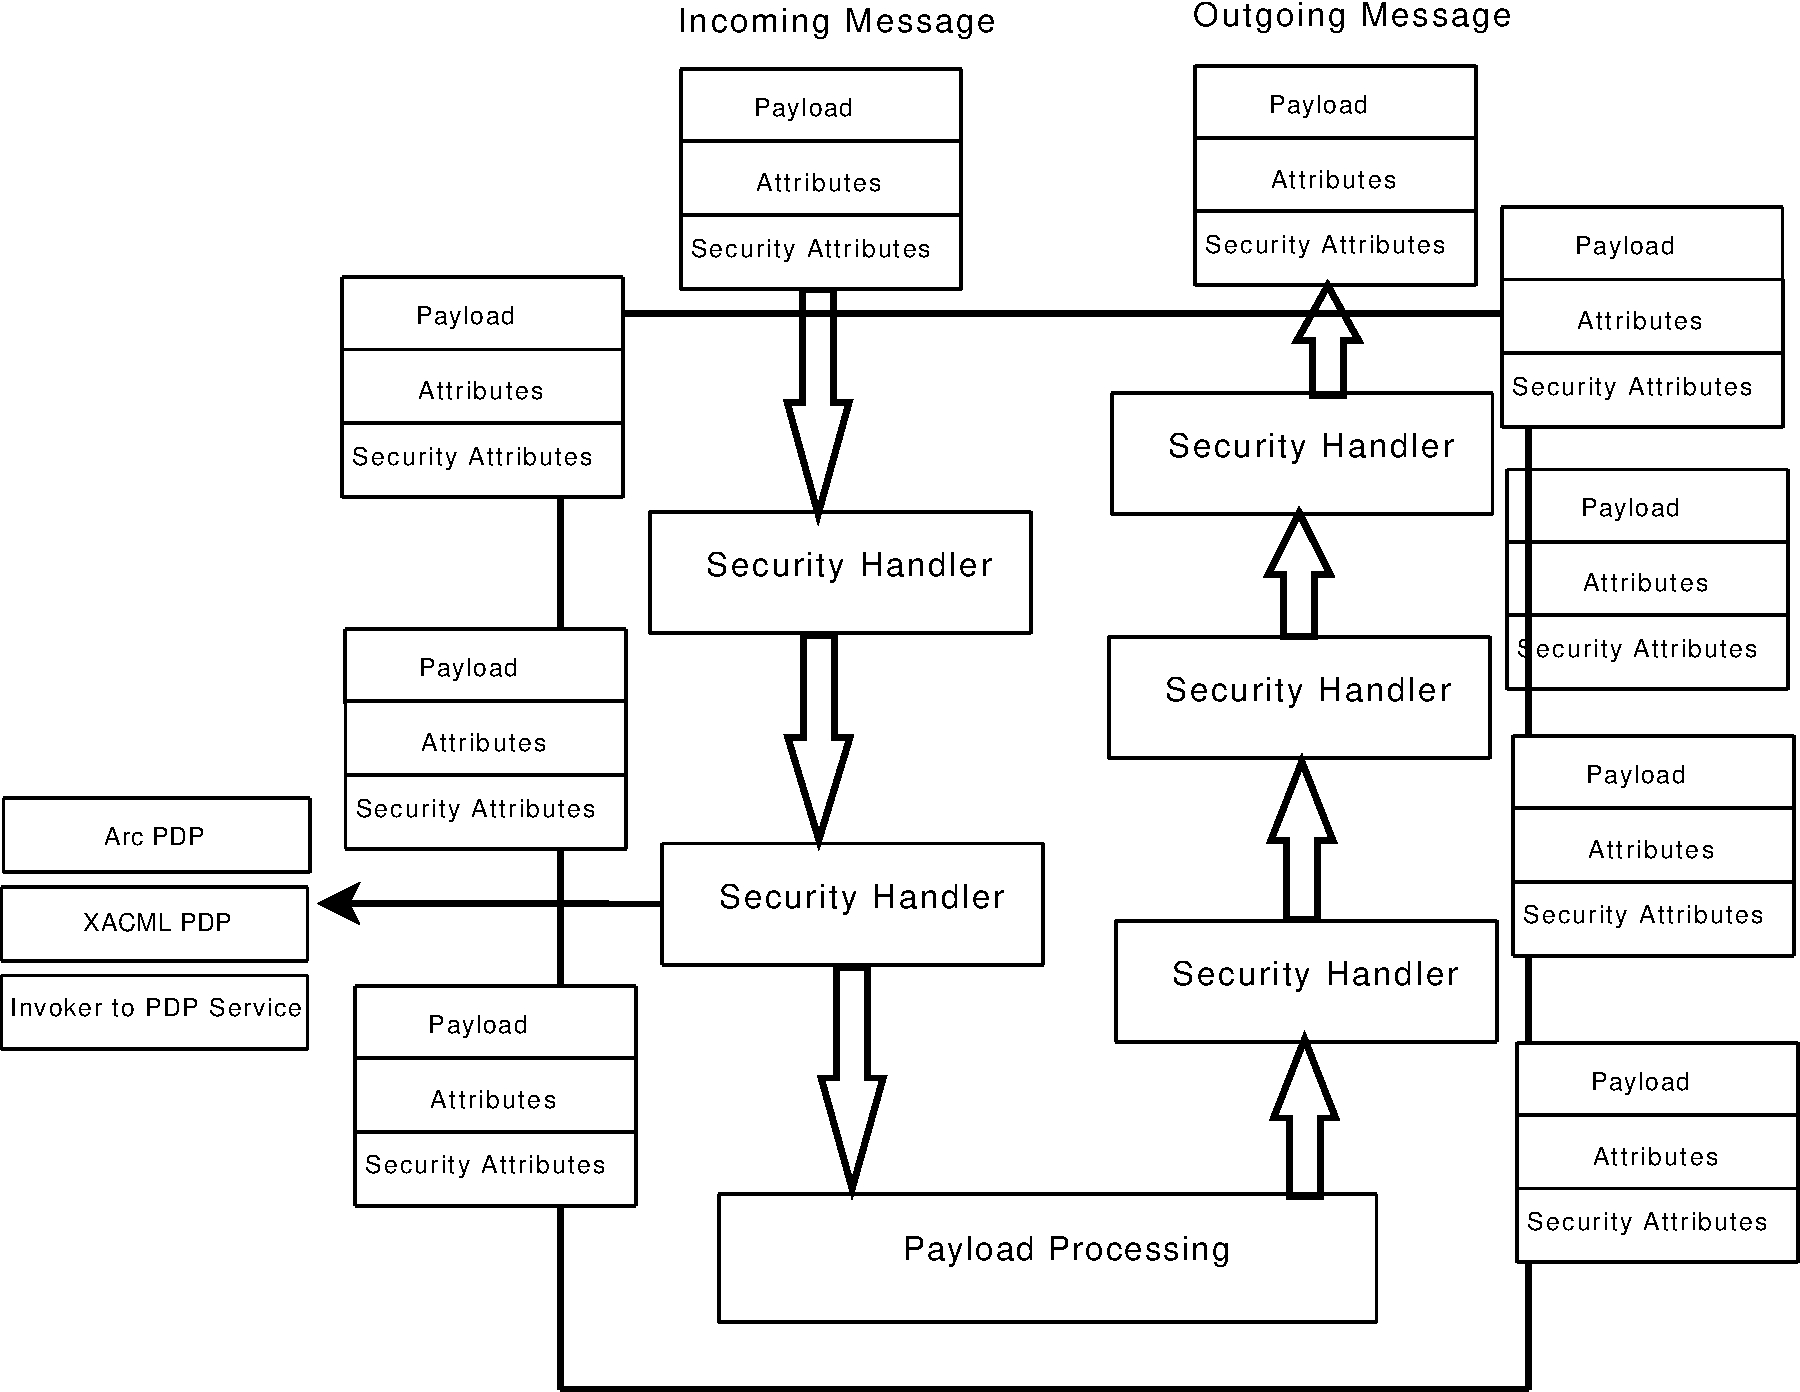
\includegraphics[width=1.0\textwidth]{MCC_Component.pdf}}}
\caption{
\label{fig:messageinMCC}
\textit{There are usually two chains of SecHandlers inside the MCC or service. Each SecHandler will parse the Security Attributes which are generated by the upstream MCC/services or probably upstream SecHandlers in the same or other MCC/Service, and do message processing or authenticate or authorize the incoming/outgoing message based on the collected information. The SecHandler can also change the payload and attributes of Messsage itself. For example, the Username-Token SecHandler will insert the WSS Username Token \cite{ws-security} into header part of SOAP message. The PDPs are called by the dedicated SecHandlers and are supposed to make authorization decision. In this example two local PDPs and one remote PDP service are presented, and any number of PDPs can be configured under corresponding SecHandler.
}} }
\end{figure}

The configuration of SecHandler components for an example ``Echo'' service is shown below. Example ``Echo'' service is configured to use two SecHandlers, both performing authorization. First SecHandler uses the X.509 identity of client (certificate subject) extracted from the incoming message to map it into local identity like Linux username. In this case all clients are mapped to local account ``test''. The second one uses two PDPs: one will compose ARC specific authorization request based on the Security Attributes collected from incoming message and evaluate it against the ARC specific authorization policy which is stored in local file ``policy.xml'', the other will compare the X.509 identity of client extracted from the incoming message against list of identities stored locally.

\begin{verbatim}
<Service name="echo" id="echo">
    <SecHandler name="identity.map" id="map" event="incoming">
        <PDP name="allow.pdp"><LocalName>test</LocalName></PDP>
    </SecHandler>
    <SecHandler name="arc.authz" id="authz" event="incoming">
        <PDP name="arc.pdp">
            <PolicyStore>
                <Location type="file">policy.xml</Location>
                <!-- other policy location-->
            </PolicyStore>
        </PDP>
        <PDP name="simplelist.pdp" location="pemittedlist.txt"/>
    </SecHandler>
</Service>
\end{verbatim}


\subsection{Interface of SecHandler} % (fold)
\label{subsec:interface_sechandler}

When either MCC or Service are loaded according to the configuration information, the SecHandler under the component and the plug-ins like PDP which are attached to the SecHandler will be loaded as well.

Each SecHandler implements one simple interface (see below), which is called by the containing MCC/Service once there is message (incoming or outgoing) need to be processed.

\begin{verbatim}
class SecHandler {
   public:
    SecHandler(Arc::Config*) {};
    virtual ~SecHandler() {};
    virtual bool Handle(Arc::Message *msg) = 0;
  };
\end{verbatim}

Class \textit{SecHandler} is an abstract class which includes a general interface method called \textit{Handle} which takes Message object as argument. Any security handler implementation must inherit from class \textit{SecHandler} and implement the interface according to the actual functionality. The method returns simple \textit{Boolean} value, and any useful information generated during the calling of this interface should be put into the security attributes of the message, or put into the payload itself.

Currently, the ARC NOX comes with the following security handlers implemented:

\begin{itemize}
    \item arc.authz Authorization SecHandler
The arc.authz and serves as container for the Policy Decision Point components. It is responsible for calling their interface and getting back the authorization result. Then obtained results are processed and combined decision is made. Description of configuration and examples can be found in section \ref{subsec:authzhandler_conf}. Usually the Authorization SecHandler and included PDPs are used on the service side of communication channel. Although it is also possible to use them on the client side.

    \item identity.map Identity Mapping SecHandler
The identity.map is a specific authorization oriented security handler. It will map the global identity in the message into local identity like system username based on the result returned by Policy Decision Point components.

    \item delegation.collector Delegation Collector SecHandler
The delegation.collector is responsible for collecting the delegation policy information from the remote proxy credential (proxy certificate compatible with RFC3820) inside the message, and putting this policy into the message security attribute for the usage of other components, such as the ``delegation.pdp''.

    \item usernametoken.handler UseranemToken SecHandler
The task of the  usernametoken.handler is to generate the WS-Security\cite{ws-security} Username Token and add it into header of SOAP message which is the payload of outgoing message. It can also extract the WS-Security Username-Token from the header of SOAP message which is the payload of incoming message.

    \item x509token.handler X.509 Token SecHandler
This SecHandler generates and process the WS-Security\cite{ws-security} X.509 Token inside the header of SOAP message.

    \item samltoken.handler 

    \item saml2ssoassertionconsumer.handler 

    \item delegation.handler 

\end{itemize}


\subsection{Interface of PDP} % (fold)
\label{subsec:interface_pdp}

Below is the definition of abstract class PDP. The implementation for example could implement method isPermitted() by composing the policy evaluation request, evaluating this request against some policy, and returning the evaluation result. Or it could compose the policy evaluation request, invoke some remote policy decision web service and return back the evaluation result.

\begin{verbatim}
class PDP {
   public:
    PDP(Arc::Config* cfg) { };
    virtual ~PDP() {};
    virtual bool isPermitted(Arc::Message *msg) = 0;
  };
\end{verbatim}

Class \textit{PDP} is an abstract class which includes a general interface method called \textit{isPermitted} which uses Message object as argument. Any policy decision point implementation must inherit from class PDP and implement the interface according to the actual functionality. The interface method return simple \textit{Boolean} value, and any useful information generated during the calling of this interface should be put into the security attribute of the message, or put into the payload itself.

Currently, the ARC NOX comes with the following PDP implementations:

\begin{itemize}
    \item arc.pdp Arc PDP
The Arc PDP will organize the security attributes into the ARC specific authorization request, call the policy evaluator to evaluate the request against the policy (which is in ARC specific format) stored in local repository, and return back the evaluation result. See section \ref{sec:policy_eval} for detailed information about request and policy schema.

    \item xacml.pdp XACML PDP
The XACML PDP will organize the security attributes into the XACML authorization request (see: http://docs.oasis-open.org/xacml/2.0/access\_control-xacml-2.0-context-schema-os.xsd), call the policy evaluator to evaluate the request against the policy (which is in XACML format: http://docs.oasis-open.org/xacml/2.0/access\_control-xacml-2.0-policy-schema-os.xsd) stored in local repository, and return back the evaluation result.

    \item delegation.pdp Delegation PDP
The Delegation PDP is basically similar to Arc PDP, except it uses the delegation policy parsed from remote proxy credential by delegation.collector, and evaluates the request against configured delegation policy. See section \ref{sec:delegation} for the design idea and use case of delegation policy in fine-grained identity delegation.

    \item simplelist.pdp Simplelist PDP
The Simplelist PDP is a simplest implementation of policy decision point. It will match the identity extracted from the remote credential (or proxy credential) to local list of permitted identities.

    \item pdpservice.invoker PDP Service Invoker
The PDP Service Invoker is a client which can be used to invoke the PDP Service which implements the same functionality as Arc PDP or XACML PDP, except that the evaluation request and response are carried by SOAP message. The benefit of implementing PDP Service and PDP Service Invoker is that the policy evaluation engine can be accessed remotely and maintained centrally.

    \item allow.pdp Allow PDP
This PDP always returns positive result.

    \item deny.pdp Deny PDP
This PDP always returns negative result.

\end{itemize}

%section sec_architecture (end)



\section{Policy Evaluation Engine} % (fold)
\label{sec:policy_eval}

\subsection{Design of policy evaluation engine} % (fold)
\label{subsec:design_policyengine}

The ARC NOX defines specific evaluation request and policy schema. Based on the schema definition, one policy evaluation engine is implemented. The design principal of policy evaluation engine is generality by which the implementation of the policy evaluation engine can be easily extended to adopt some other policy schema, such as XACML policy schema.

\begin{figure}[ht]
\centering{{{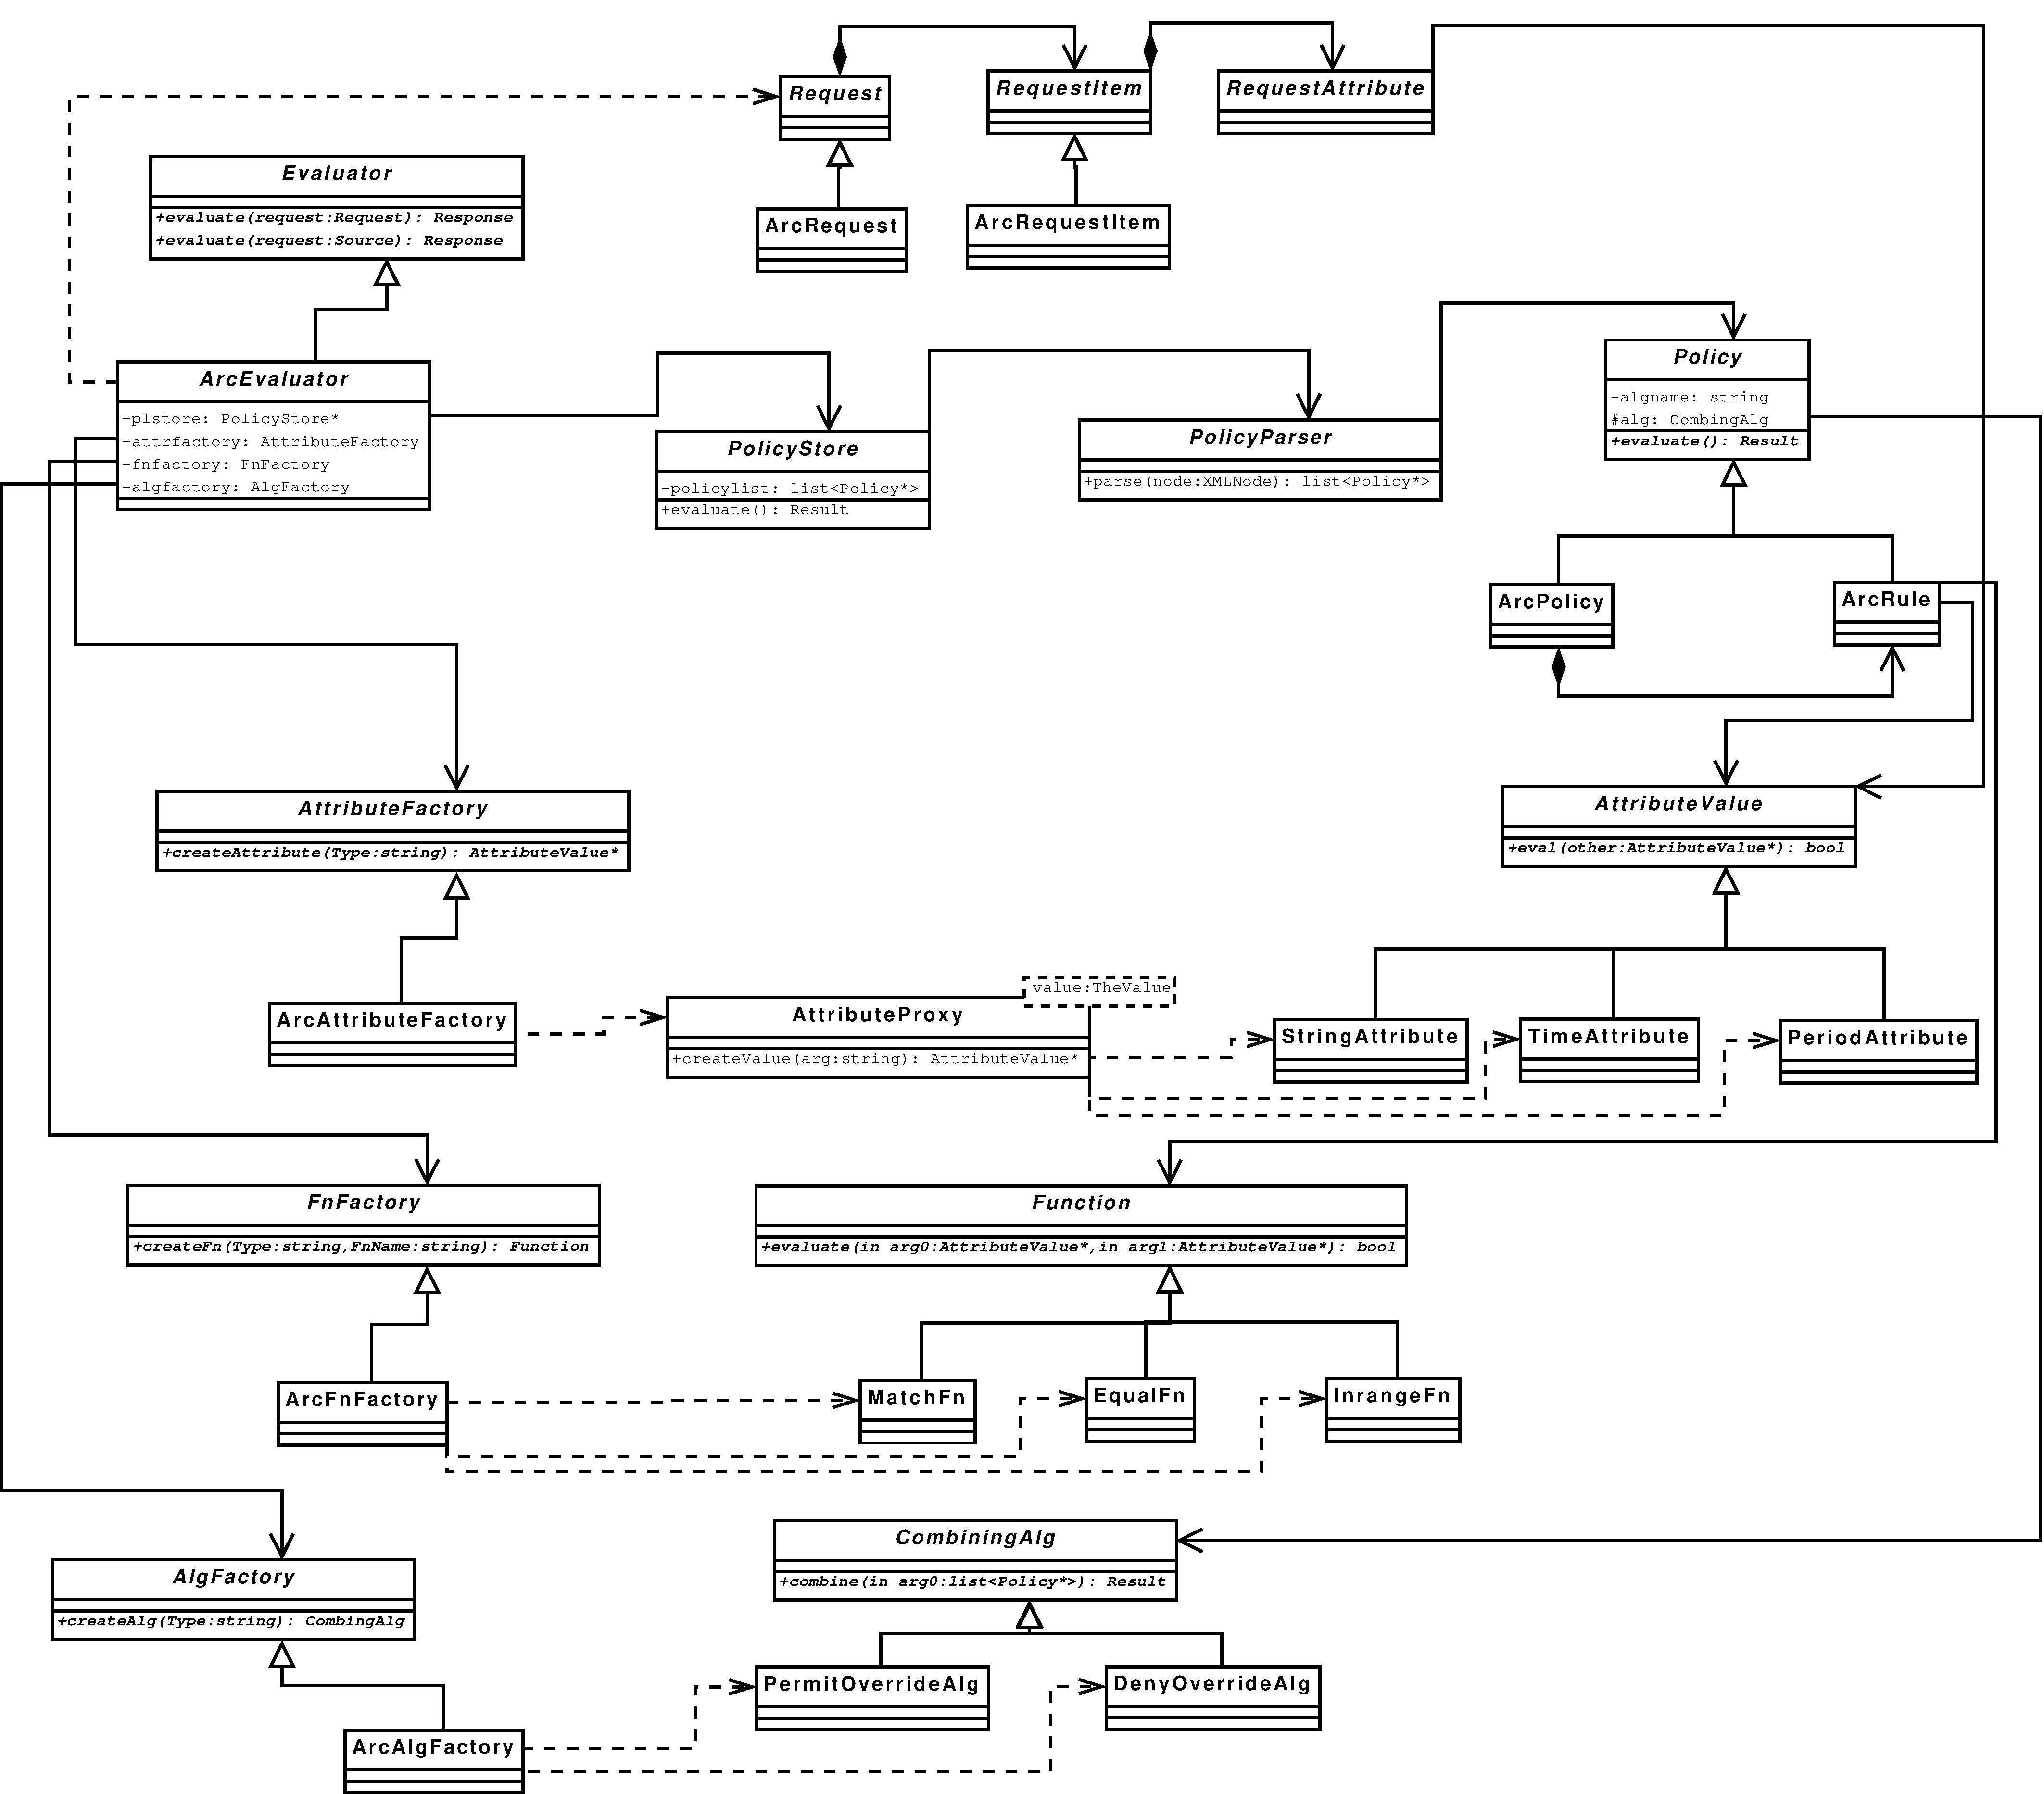
\includegraphics[width=1.0\textwidth]{Evaluator_ARC.pdf}}}
\caption{\label{fig:policyengine_ARC}The UML class diagram of the classes inside policy evaluation engine that support ARC policy} }
\end{figure}

\begin{figure}[ht]
\centering{{{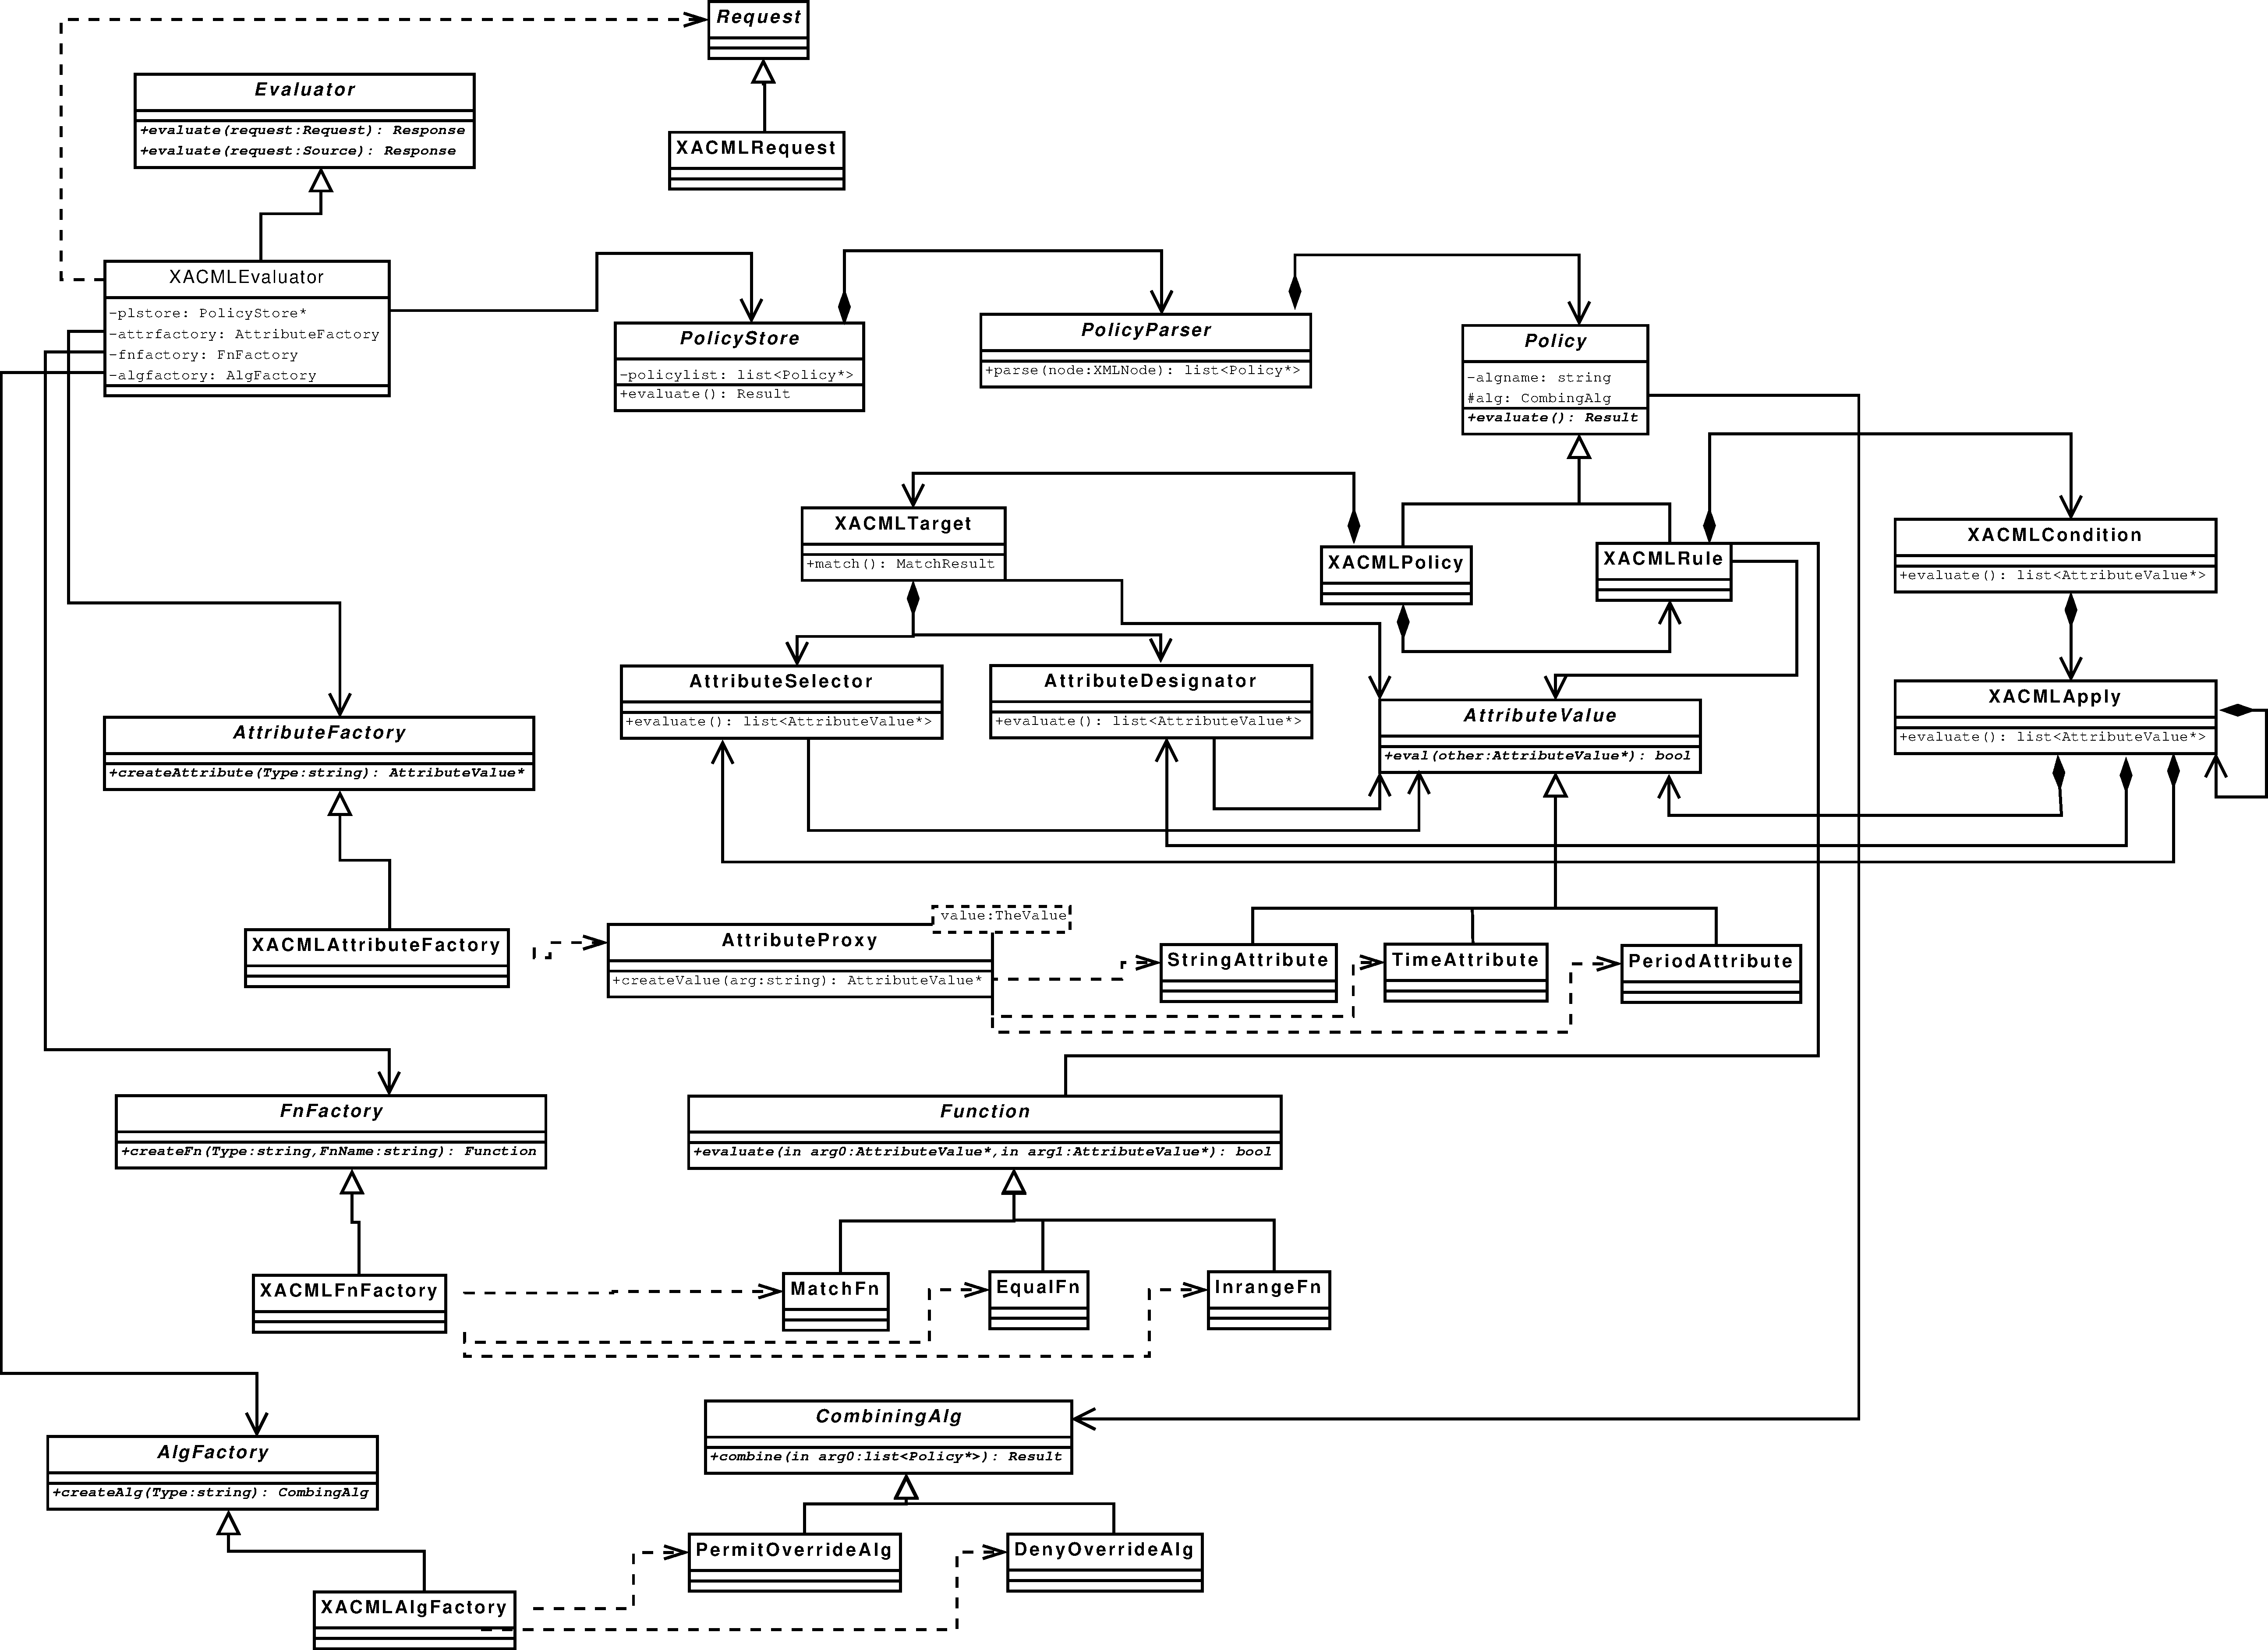
\includegraphics[width=1.0\textwidth]{Evaluator_XACML.pdf}}}
\caption{\label{fig:policyengine_XACML}The UML class diagram of the classes inside policy evaluation engine that support XACML policy} }
\end{figure}

Figure \ref{fig:policyengine_ARC} and \ref{fig:policyengine_XACML} respectively show the UML class diagram about the policy evaluation engine for ARC policy and XACML policy. They show all classes and relations simultaneously for getting the overall picture.


The \textbf{Evaluator} class is the key class for policy evaluation. It accepts request evaluates it against loaded policy and returns evaluation response.

Three abstract factories - \textit{FnFactory}, \textit{AlgFactory}, \textit{AttributeFactory} - are responsible for creating the \textit{Function}, \textit{CombiningAlg} and \textit{AttributeValue} objects correspondingly. The classes inherited from \textit{CombiningAlg} class take care of implementing various combining algorithms which define relations between \textit{$<$Rule/$>$} elements in policy. The \textit{AttributeValue} type of classes are used for processing different types of \textit{$<$Attribute/$>$} and similar elements. The \textit{Function} classes take care of comparing \textit{$<$Attribute/$>$} elements of request and policy.

The \textit{Policy} class parses \textit{$<$Policy/$>$} or \textit{$<$Rule/$>$} elements and creates \textit{CombingAlg} objects according to the \textit{$<$RuleCombiningAlg/$>$} attribute of \textit{$<$Policy/$>$}, \textit{Function} objects according to the \textit{$<$Function/$>$} attribute of \textit{$<$Attribute/$>$} and \textit{AttributeValue} objects according to the \textit{$<$Type/$>$} attribute of \textit{$<$Attribute/$>$}. Those objects will be used when evaluating the request.

The \textit{Request} class is responsible for parsing \textit{$<$Request/$>$} element and creates corresponding \textit{AttributeValue} objects according to the \textit{$<$Type/$>$} attribute of \textit{$<$Attribute/$>$}. When evaluating, each \textit{AttributeValue} in request will be evaluated against corresponding \textit{AttributeValue} in the policy by using relevant \textit{Function}.

Due to extensible architecture of code it is relatively easy to add support for new types of \textit{AttributeValue}, \textit{Function} and \textit{CombingAlg} objects in this way supporting various types of XML based policy languages.

\subsection{Policy evaluation engine --- Support of ARC policy and request} % (fold)
\label{subsec:policy_engine_arc}


\subsubsection{Schemas for ARC policy and request} % (fold)
\label{subsubsec:arc_policy_schema}
The schema for ARC Policy is available at

http://svn.nordugrid.org/trac/nordugrid/browser/arc1/trunk/src/hed/pdc/arcpdp/Policy.xsd .

The hierarchy tree of ARC Policy is shown below (numbers show multiplicity of elements)

\begin{verbatim}
    Policy (1)
        Rule (1-)
            Subjects (1)
                Subject (1-)
                    Attribute (1-)
            Resources (0-1)
                Resource (1-)
            Actions (0-1)
                Action (1-)
            Conditions (0-1)
                Condition (1-)
                    Attribute (1-)
\end{verbatim}

The schema for ARC Request is available at

http://svn.nordugrid.org/trac/nordugrid/browser/arc1/trunk/src/hed/pdc/arcpdp/Request.xsd .

The hierarchy tree of ARC Request is show below (numbers show multiplicity of elements)

\begin{verbatim}
    Request (1)
        RequestItem (1-)
            Subject (1-)
          SubjectAttribute (1-)
            Resource (0-)
            Action (0-)
            Context (0-)
                ContextAttribute (1-)
\end{verbatim}


The schema for ARC Response is available at

http://svn.nordugrid.org/trac/nordugrid/browser/arc1/trunk/src/hed/pdc/arcpdp/Response.xsd .

The ARC Response is not used directly in code. It is in use by PDP Service which provides remote evaluation of policies.


\subsubsection{Basic Elements of Policy} % (fold)
\label{subsubsec:poicy_element}
There are 2 basic objects - ``policy'' and ``request''. There is 1 main actor - Evaluator. Curretly there are two types of elements in policy: \textit{Policy} and \textit{Rule}. \textit{Policy} element is made of \textit{Rule} elements.
\textit{Evaluator} matches request to policy and produces one of 4 following results:

\begin{itemize}
    \item  \emph{PERMIT} - policy explicitely permits activity specified in request because request matches some part of policy and corresponding effect specified in policy is PERMIT.

        \emph{Example}:

            \emph{Rule}: PERMIT person ALICE to PLAY in place called WONDERLAND

            \emph{Request}: person ALICE wants to PLAY in place called WONDERLAND

    \item  \emph{DENY} - policy explicitely denies activity specified in Request because Request matches some part of policy and corresponding effect specified in policy is DENY.

        \emph{Example}:

            \emph{Rule}: DENY fruit APPLE to GROW on PEACH tree

            \emph{Request}: fruit APPLE to be GROWN on PEACH tree

    \item  \emph{INDETERMINATE} - request has some part which does not correspond to policy.

        \emph{Example}:

            \emph{Rule}: DENY fruit APPLE to GROW on PEACH tree

            \emph{Request}: fruit APPLE to be GROWN on WHEAT ground

            \emph{Request}: flower SUNFLOWER to be grown on PEACH tree

        \emph{Explaination}: Here, it is not possible to obtain any matching result - neither positive (DENY or PERMIT) nor negative (NOT\_APPLICABLE, see below)

In the request, the ``ground'' is completely uncomparable to the ``tree'' in policy. One can compare ``PEACH tree'' and ``APPLE tree'' because they are both ``tree''; But it is impossible to compare ``PEACH tree'' and ``WHEAT ground'' becaue they of different kind (Policy is about tree and Request is about ground).

In a similar way one can't compare ``fruit APPLE'' and ``flower SUNFLOWER'' (here policy is about fruits and Request is about flower).

Any other situation which makes it impossibile to compare two attributes will also cause ``INDETERMINATE''.

    \item  \emph{NOT\_APPLICABLE} - all parts of the Request have corresponding parts in the Policy, but some value of those parts are not the same. Hence request does not match policy.

        \emph{Example}:

            \emph{Rule}: DENY fruit APPLE to GROW on PEACH tree

            \emph{Request}: fruit APPLE to be GROWN on APPLE tree

            \emph{Request}: fruit ORANGE to be GROWN on PEACH tree

            \emph{Request}: fruit ORANGE to be GROWN on APPLE tree

        \emph{Explanation}: for each part of the Request evaluator can find relevant part in the Policy - both Policy and Request are about fruit and tree. But the values do not match.

\end{itemize}

If it is required to reduce evaluation results to boolean value PERMIT maps to TRUE and rest of results to FALSE.

\emph{Note}: It would be useful to make it possible to specify secondary effect which would become active in case Request is NOT\_APPLICABLE. For example:

DENY fruit APPLE to GROW on PEACH tree otherwise PERMIT

But one should be careful because example above would allow fruit PLUMS to grow on APPLE trees :)

This kind of requirement can be supported by using the algorithm between policies.  For example, in case of above scenario, we can use some algorithm like "Permit-if-notapplicable". See below the "Policy matching" part for more explaination.


\subsubsection{Policy Matching} % (fold)
\label{subsubsec:poicy_matching}
Policy is made of Rule elements. Request is evaluated against each Rule. Each evaluation produces same results as policy evaluation described above. The results from all Rules are then combined in order to produce final result for whole policy. Results Combining Algorithm is specified in Policy. There are 26 algorithms currently:

\begin{itemize}
    \item  \emph{Deny-Overrides} - this is default if no algorithm specified.

    \begin{itemize}
        \item If there is at least one DENY in results final result is DENY.
        \item Otherwise if there is at least one PERMIT, the final result is PERMIT.
        \item Otherwise if there is at least one NOT\_APPLICABLE final result is NOT\_APPLICABLE.
        \item Otherwise final result is INDETERMINATE.
    \end{itemize}

    Special case is Policy with no rules. Probably such policy should be treated as always producing DENY.

    \item  \emph{Permit-Overrides}

    \begin{itemize}
        \item If there is at least one PERMIT in results final result is PERMIT.
        \item Otherwise if there is at least one DENY the final result is DENY.
        \item Otherwise if there is at least one NOT\_APPLICABLE final result is NOT\_APPLICABLE.
        \item Otherwise final result is INDETERMINATE.
    \end{itemize}

    Special case is Policy wih no rules. Probably such policy should be treated as always producing DENY.

    \item  \emph{Ordered algorithms}

These specify priorities for all four possible results. Their names look like Result1-Result2-Result3-Result4 with Result\# naming result types, for example Permit-Deny-NotApplicable-Indeterminate. The results are combined in following way:

    \begin{itemize}
        \item If there is at least one result of Result1 type then final result is Result1.
        \item Otherwise if there is at least one result of Result2 type then final result is Result2.
        \item Otherwise if there is at least one result of Result3 type then final result is Result3.
        \item Otherwise final result is Result4.
    \end{itemize}

    There are 24 possible combinations of those algorithms.

\emph{Note}: It would be useful to have more combining algorithms. For example

    \item  \emph{Permit-if-notapplicable} - the use case could be ``DENY fruit APPLE to GROW on PEACH tree otherwise PERMIT''. In this case there is only one Rule under Policy, and this Rule is with ``Deny'' effect.

    \begin{itemize}
        \item If this Rule gives DENY in results, final result is DENY.
        \item Otherwise if this Rule gives NOT\_APPLICABLE, final result is PERMIT.
        \item Otherwise final result is INDETERMINATE.
    \end{itemize}

    \item  \emph{Permit-if-allPermit} - Permit if all the Rules gives Permit, this algorithm is useful in case if we are collecting different policies from a few sources, and we want the request to satisfy all of them.

    \begin{itemize}
        \item If all of the Rule give PERMIT, the final result is PERMIT.
        \item Otherwise if there is at least one DENY the final result is DENY.
        \item Otherwise if there is at least one NOT\_APPLICABLE final result is NOT\_APPLICABLE.
        \item Otherwise final result is INDETERMINATE.
    \end{itemize}

    \item  \emph{OnlyOneApplicable}

    \begin{itemize}
        \item If there is one gives INDETERMINATE, final result INDETERMINATE is given immediately.
        \item Otherwise if there is exactly only one gives applicable result (DENY or PERMIT), final result is as this result.
        \item Otherwise if there is more than one gives applicable result, final result is INDTERMINATE.
        \item Otherwise final result is NOT\_APPLICABLE.
    \end{itemize}

This algorithm makes sure that only one Rule is selected when making decision.

    \item  \emph{FirstApplicable}

    \begin{itemize}
        \item If there is one give DENY, PERMIT or INDETERMINATE result, final result is given immediately as this result.
        \item Otherwise final result is NOT\_APPLICABLE.
    \end{itemize}

\end{itemize}


\subsubsection{Request Structure} % (fold)
\label{subsubsec:request_structure}

Request is made of RequestItem elements. Each RequestItem is evaluated against Policy Rule and for each evaluation separate result is generated as described above.RequestItem is made of 4 elements:
    \begin{itemize}
        \item \emph{Subject} - represents entity requesting specified action
        \item \emph{Resource} - destination/object of the action
        \item \emph{Action} - specifies what has to be done on resource
        \item \emph{Context} - for additional information which does not fit anywhere else, like the current time.
    \end{itemize}

Effectively RequestItem may have only one Subject, one Resource, one Action and one Context. If there are more than one element of any kind of sub-elelemt, then in the evaluator this RequestItem is split into several items containing all possible permutations and results are obtained for every item separately. How results are combined will be explained later.
Additionally Subject could contain sub-elements SubjectAttribute. Those are meant to represent different kinds of requesters' identities. Example:

    \begin{itemize}
        \item Subject
        \begin{itemize}
            \item SubjectAttribute: name is ALICE
            \item SubjectAttribute: age is YOUNG
            \item SubjectAttribute: gender is GIRL
        \end{itemize}
    \end{itemize}
Context could also be made of ContextAttribute elements in the same way as Subject.

The following is an example of the Request:

\begin{verbatim}
    <Request xmlns="http://www.nordugrid.org/schemas/request-arc">
        <RequestItem>
            <Subject>
                <SubjectAttribute AttributeId="urn:knowarc:x509:identity">
                    /O=KnowARC/OU=UiO/CN=Physicist
                </SubjectAttribute>
                <SubjectAttribute AttributeId="urn:knowarc:voms:attribute>
                    knowarc:atlasuser
                </SubjectAttribute>
            </Subject>
            <Subject AttributeId="urn:knowarc:shibboleth:attribute">member</Subject>
            <Action AttributeId="urn:knowarc:fileoperation">Read</Action>
            <Resource AttributeId="urn:knowarc:fileidentity>file:///home/test</Resource>
            <Context AttributeId="urn:knowarc:time" Type="time">2008-09-15T20:30:20</Context>
        </RequestItem>
    </Request>
\end{verbatim}

While evaluating this RequestItem will be split into two RequestItems:

\begin{verbatim}
    <Request xmlns="http://www.nordugrid.org/schemas/request-arc">
        <RequestItem>
            <Subject>
                <SubjectAttribute AttributeId="urn:knowarc:x509:identity">
                    /O=KnowARC/OU=UiO/CN=Physicist
                </SubjectAttribute>
                <SubjectAttribute AttributeId="urn:knowarc:voms:attribute>
                    knowarc:atlasuser
                </SubjectAttribute>
            </Subject>
            <Action AttributeId="urn:knowarc:fileoperation">Read</Action>
            <Resource AttributeId="urn:knowarc:fileidentity>file:///home/test</Resource>
            <Context AttributeId="urn:knowarc:time" Type="time">2008-09-15T20:30:20</Context>
        </RequestItem>
        <RequestItem>
            <Subject AttributeId="urn:knowarc:shibboleth:attribute">member</Subject>
            <Action AttributeId="urn:knowarc:fileoperation">Read</Action>
            <Resource AttributeId="urn:knowarc:fileidentity>file:///home/test</Resource>
            <Context AttributeId="urn:knowarc:time" Type="time">2008-09-15T20:30:20</Context>
        </RequestItem>
    </Request>
\end{verbatim}

The following means this Subject possesses both of these Attributes.

\begin{verbatim}
    <Subject>
        <SubjectAttribute AttributeId="urn:knowarc:x509:identity">
            /O=KnowARC/OU=UiO/CN=Physicist
        </SubjectAttribute>
        <SubjectAttribute AttributeId="urn:knowarc:voms:attribute>
            knowarc:atlasuser
        </SubjectAttribute>
    </Subject>
\end{verbatim}

However, the following means two Subject each of which possesses one Attribute.

\begin{verbatim}
    <Subject AttributeId="urn:knowarc:x509:identity">
        /O=KnowARC/OU=UiO/CN=Physicist
    </Subject>
    <Subject AttributeId="urn:knowarc:voms:attribute>
        knowarc:atlasuser
    </Subject>
\end{verbatim}

The ``Type'' xml-attribute is for distinguishing how to process the xml-node value, which is critical when evaluate two value from request side and policy side because different type requires different evaluating/comparing approach. The default ``Type'' is ``string'', in this case (also with the ``Function'' xml-attribute on the policy side is ``equal'', which will be explained later), each letters of these two values will be compared one by one when evaluating them.

The ``AttributeId'' xml-attribute is for evaluator to find the Attribute with AttributeId from the request side which corresponds to the Attribute with the same AttributeId on the policy side. Only if two Attributes' AttributeId are equal, the evaluator will then compare the value.

Each RequestItem will be sequencialy and independently evaluated against policy/policies. So for one Request (including few RequestItems), some RequestItem could get positive evaluation result (PERMIT) from policy engine, others could get negative evaluation result (DENY, NOT\_APPLICABLE, INDETERMINATE).

It is up to policy decision point to make final decision according to the evaluation results returned by evaluator, and the evaluator itself can not give this kind of final decision.

Basically the policy decision point will feed policy engine with request, get back evaluation results,
and make final decision.


\subsubsection{Rule Composition and Matching} % (fold)
\label{subsubsec:rule_comp_match}

Policy rule is made of 4 elements - Subjects, Resources, Actions, Conditions (See the following example). Those are only used to group multiple elements Subject, Resource, Action, Condition. For instance, you can merge two Rules with the same Resources, Actions, Conditions, and the same ``Effect'' but different Subjects into one Rule.

There is no logical relationship between Subject, which means you can split one Rule into two Subject (under Subjects) into two Rule (each of which has one Subject (under Subjects)).From now only later ones (Subjects with only one Subject as sub-element, and the same for others) are described. Their meaning is same as in request with Condition corresponding to Context. Subject and Condition elements are also made of Attributes. All elements may be present more than one time. During procedure of matching each element in RequestItem is matched against all elements of same kind in Policy - Subject is matched to Subject, Resource to Resource, etc. For every combination 3 possible results are produced:

    \begin{itemize}
        \item \emph{MATCHED} - element from RequestItem matched element in Policy Rule.
            \emph{Example}:
            \emph{RequestItem Resource}: \textit{place called WONDERLAND}
            \emph{PolicyItem Resource}: \textit{place called WONDERLAND}
        \item \emph{NOT MATCHED} - element from RequestItem did not match element in Policy Rule.
            \emph{Example}:
            \emph{RequestItem Resource}: \textit{place called WONDERLAND}
            \emph{PolicyItem Resource}: \textit{place called PLAYGROUND}
        \item \emph{INDETERMINATE} - element from RequestItem could not be compared to element in Policy  Rule because they are of incompatible ids/belong to different namespaces.
            \emph{Example}:
            \emph{RequestItem Resource}: \textit{place called WONDERLAND (with namespace ``place'')}
            \emph{PolicyItem Resource}: \textit{LEMON tree (with namespace ``tree'')}
    \end{itemize}

The produced results then combined to produce final 4 types of results in following way:

    \begin{itemize}
        \item If for every element in RequestItem there is at least one MATCHED result then result for this Policy Rule is as specified in the corresponding Effect (Deny or Permit).
        \item Otherwise if for every element in RequestItem there is at least one gets INDETERMINATE result then result for Policy Rule is INDETERMINATE.
        \item Otherwise result is NOT\_APPLICABLE.
    \end{itemize}

Special case is then RequestItem does not have the element(s) of some kind (Subject, Action, Resource or Context/Condition). If there are elements of corresponding kind in the Policy Rule then such situation should be considered as INDETERMINATE.

The following is an example of the Policy:

\begin{verbatim}
<Policy xmlns="http://www.nordugrid.org/schemas/policy-arc" CombiningAlg="Permit-Overrides">
    <Rule Effect="Permit">
        <Subjects>
            <Subject>
                <Attribute AttributeId="urn:knowarc:x509:identity">
                    /O=KnowARC/OU=UiO/CN=Physicist
                </Attribute>
                <Attribute AttributeId="urn:knowarc:voms:attribute>
                    knowarc:atlasuser
                </Attribute>
            </Subject>
            <Subject AttributeId="urn:knowarc:shibboleth:attribute">member</Subject>
        </Subjects>
        <Actions>
            <Action AttributeId="urn:knowarc:fileoperation">Read</Action>
            <Action AttributeId="urn:knowarc:fileoperation">Delete</Action>
        </Actions>
        <Resources>
            <Resource AttributeId="urn:knowarc:fileidentity">file:///home/test</Resource>
        </Resources>
        <Conditions>
            <Condition AttributeId="urn:knowarc:period" Type="period" Function="Inrange">
                2008-09-10T20:30:20/P1Y1M
            </Condition>
        </Conditions>
    </Rule>
</Policy>
\end{verbatim}

For the Subject which includes two Attributes in this example:

\begin{verbatim}
    <Subject>
        <Attribute AttributeId="urn:knowarc:x509:identity">
            /O=KnowARC/OU=UiO/CN=Physicist
        </Attribute>
        <Attribute AttributeId="urn:knowarc:voms:attribute>knowarc:atlasuser</Attribute>
    </Subject>
\end{verbatim}

These two attributes mean the Rule requires the request should possess both of these two attributes.

However, if You put these above two Attribute into two Subject elements:

\begin{verbatim}
    <Subject AttributeId="urn:knowarc:x509:identity">/O=KnowARC/OU=UiO/CN=Physicist</Subject>
    <Subject AttributeId="urn:knowarc:voms:attribute>knowarc:atlasuser</Subject>
\end{verbatim}

Then it means the Rule requires the request to possess at least one of these two attributes.

For the xml-attribute ``Type'' and ``AttributeId'', the explaination for Request example also applies here.
The ``Function'' xml-attribute is for distinguishing different comparison algorithm when comparing these two xml-node value. If Function is absent, ``equal'' will be used as default.


\subsubsection{Rule Elements Matching} % (fold)
\label{subsubsec:rule_element_match}
For elements without attributes those elements have:

    \begin{itemize}
        \item Kind specified by AttributeId XML attribute. There is no default.
        \item Matching algorithm specified by Id XML attribute. By default string-equal matching is used.
        \item Content

        \textit{Example}: LEMON tree

        \textbf{Kind}: tree

        \textbf{Matching algorithm}: default

        \textbf{Content}: LEMON

    \end{itemize}

Matching procedure consists of following steps:
    \begin{itemize}
        \item Kinds are compared using simple string equal matching. If those do not match then result is INDETERMINATE.
        \item Matching algorithm is used to compare content of elements. Result is either MATCH or NO\_MATCH according to matching algorithm.
    \end{itemize}

Each element on the RequestItem must satisfy corresponding element in Rule.In detail, for Subjects element under Rule, if there is at least one Subject (with one Attribute or a few Attribute) which is matched by a Subject on this RequestItem, we say this Subjects is matched by the RequestItem; and also the same for the other elements (Actions, Resources, Conditions).

For elements with multiple Attribute sub-elements the way to judging whether elements match is if and only if all of the Attribute under the Rule have matching Attributes at RequestItem side.

Example of the Subject with three Attributes:

    \textbf{Subject}:

    \textbf{SubjectAttribute}: name is ALICE

    \textbf{SubjectAttribute}: age is YOUNG

    \textbf{SubjectAttribute}: gender is GIRL

In XML that is:

\begin{verbatim}
    <Subject>
        <Attribute AttributeId="name">Alice</Attribute>
        <Attribute AttributeId="age>YOUNG</Attribute>
        <Attribute AttributeId="gender>GIRL</Attribute>
    </Subject>
\end{verbatim}

That requires the Subject in the RequestItem to possess at least these three Attributes.

\begin{verbatim}
    <RequestItem>
        <Subject>
            <Attribute AttributeId="name">Alice</Attribute>
            <Attribute AttributeId="age">YOUNG</Attribute>
            <Attribute AttributeId="gender">GIRL</Attribute>
        <!--Some other Attribute-->
        </Subject>
    </RequestItem>
\end{verbatim}

The above example shows that the Subject in the RequestItem ``MATCH'' one Subject on the Rule side.

If the Subject in the RequestItem is like this:

\begin{verbatim}
    <Subject>
        <Attribute AttributeId="name">Alice</Attribute>
        <Attribute AttributeId="age>YOUNG</Attribute>
        <Attribute AttributeId="from">OSLO</Attribute>
        <!--Some other Attribute, buts not a "gender"-->
    </Subject>
\end{verbatim}

Then evaluator will produce INDETERMINATE as the match-making result of this Subject.

If the Subject in the RequestItem is like this:

\begin{verbatim}
    <Subject>
      <Attribute AttributeId="name">Bob</Attribute>
      <Attribute AttributeId="age>YOUNG</Attribute>
      <Attribute AttributeId="gender">BOY</Attribute>
      <!--Some other Attribute-->
    </Subject>
\end{verbatim}

Then evaluator will give NO\_MATCH as the match-making result of this Subject.

Finally if and only if all of the elemens (Subjects, Actions, Resources, Conditions) which are not empty under the Rule have been matched (gets MATCH) to the RequestItem, then the whole Rule is considered to be matched (produces MATCH result). MATCH is then mapped to final evaluation result depending on the specified Effect. If Effect is set to Deny then DENY decision will be produced for this Rule; if Effect is Permit then PERMIT.

Otherwise if any of the element (Subjects, Actions, Resources, Conditions) of RequestItem got INDETERMINATE decision then the INDETERMINATE decision will be made for this Rule.

Otherwise the NOT\_APPLICABLE decision will be made for this Rule. In other words that means at least one of the elements of this Rule got NO\_MATCH and the other elements got MATCH.

\subsection{Policy evaluation engine --- Support of XACML policy and request} % (fold)
\label{subsec:policy_engine_xacml}
Currently, XACML specification is partially supported/implemented in ARC. More specifically, except the \textit{$<$Obligation$>$} element, other elements are supported.

http://docs.oasis-open.org/xacml/2.0/access\_control-xacml-2.0-core-spec-os.pdf

http://docs.oasis-open.org/xacml/2.0/access\_control-xacml-2.0-policy-schema-os.xsd

http://docs.oasis-open.org/xacml/2.0/access\_control-xacml-2.0-context-schema-os.xsd


\subsection{Interface for using the policy evaluation engine} % (fold)
\label{subsec:interface_policy_engine}

For making usage of policy evaluation engine more convenient basic \textit{Evaluator} class is complemented by additional interfaces. Below are examples of steps needed to carry out policy evaluation and corresponding helper interfaces.

a)Create the policy evaluation object:

\begin{verbatim}
    // Create object which provides an interface
    // for loading other objects
    ArcSec::EvaluatorLoader eval_loader;
    //Load the Evaluator
    ArcSec::Evaluator* eval = NULL;
    // Define name of policy evaluator.
    // This one is for evaluation ARC policies
    std::string evaluator = "arc.evaluator";
    // If xacml evaluation engine is used,
    // std::string evaluator = "xacml.evaluator";

    eval = eval_loader.getEvaluator(evaluator);
\end{verbatim}
b)Create the policy object:

\begin{verbatim}
    ArcSec::Policy* policy = NULL;
    // Define type of policy – ARC policy in this case
    std::string policyclassname = "arc.policy";
    // If xacml policy is used,
    // std::string policyclassname = "xacml.policy";

    // Define source from which policy to be taken
    ArcSec::SourceFile policy_source("Policy_Example.xml");
    // Load and parse policy
    policy = eval_loader.getPolicy(policyclassname, policy_source);
\end{verbatim}

c)Create the request:
\begin{verbatim}
    ArcSec::Request* request = NULL;
    // Define type of request – ARC request in this case
    std::string requestclassname = "arc.request";
    // If xacml request is used,
    // std::string requestclassname = "xacml.request";

    // Define source from which request to be taken
    ArcSec::SourceFile request_source("Request.xml");
    // Load and parse request
    request = eval_loader.getRequest(requestclassname, request_source);
\end{verbatim}

d)Add the policy into Evaluator object:
\begin{verbatim}
    eval->addPolicy(policy);
\end{verbatim}

e)Evaluate the request object:
\begin{verbatim}
    ArcSec::Response *resp = NULL;
    resp = eval->evaluate(request);
\end{verbatim}

The steps d) and e) can also be replaced by:

\begin{verbatim}
    resp = eval->evaluate(request, policy);
\end{verbatim}

The Evalutor::evaluate() method can also be feed up with both \textit{Policy}/\textit{Request} objects and their sources in any combination. See example code at http://svn.nordugrid.org/trac/nordugrid/browser/arc1/trunk/src/hed/shc/testinterface\_arc.cpp or http://svn.nordugrid.org/trac/nordugrid/browser/arc1/trunk/src/hed/shc/testinterface\_xacml.cpp for more details about usage of the interface.

The description of mentioned classes and their methods are avaialble in  API document at

http://svn.nordugrid.org/trac/nordugrid/browser/arc1/trunk/doc/KnowARC-API.pdf?format=raw .

%section policy_eval (end)


\section{Policy Decision Service (Charon Service)} % (fold)
\label{sec:policy_decision_service}
Policy decision service is a service implementation which configurably contains the functionality of ArcPDP or XACMLPDP. It will accept the soap request containing policy decision request and return soap response containing policy decision response.

The WSDL description of policy decision service is available at

 http://svn.nordugrid.org/trac/nordugrid/browser/arc1/trunk/src/services/charon/charon.wsdl

It's configuration is presented in section \ref{subsec:pdpservice_conf}.

%section policy_decision_service (end)


\section{Security Attributes -- how to compose policy decision request to policy evaluation engine} % (fold)
\label{sec:sec_attributes}

\subsection{Infrastructure} % (fold)
\label{subsec:sec_attr_infrastructure}

Security Attributes represent security related information inside HED framework and store information representing various aspects needed to perform authorization decison - identity of client, requested action, targeted resource, constraint policies.

Each kind of Security Attribute is represented by own class inherited from parent SecAttr class $<$arc/message/SecAttr.h$>$.

Each Security Attribute stores it's information in internal format and is capable to export it to one of predefined formats using \textit{Export()} method. Currently only supported format is ARC Policy/Request XML document described in sections \ref{subsec:authz_policy} and \ref{subsec:authz_request}.
Collectors of Security Attributes instantiate corresponding classes and link them to Secuirity Attributes containers - MessageAuth $<$arc/message/MessageAuth.h$>$ and MessageAuthContext $<$arc/message/Message.h$>$ storing collected attributes per request and per session correspondingly. Each attribute is assigned a name. Current implementations of Security Attributes Collectors are either integrated into existing MCCs or implemented as separate SecHandler plugins. See section \ref{subsec:sec_attr_avail_collectors} for available Collectors and corresponding Security Attributes.

Note for service developers: Services may implement own authorization algorithms. But they may use Security Atributes as well by providing instances of classes inherited from SecAttr and running them through either configured or hardcoded processors/PDPs.
Processors of Security Attributes are implemented as Policy Decision Point components. Currently there are 2 PDP components available:
Arc PDP makes use of Security Attributes containing identities of client, resource and requested action. It evaluates either all or selected set of attributes against specified Policy documents thus making it possible to enforce policies defined/selected by service providers.
Delegation PDP is described below in section \ref{subsec:delegation_pdp}.


\subsection{Available collectors} % (fold)
\label{subsec:sec_attr_avail_collectors}

Here Security Attribute collectors distributed as part of the ARC NOX are described except those used for Delegation Restrictions. Those are described in section \ref{subsec:delegation_collector}

\subsubsection{TCP} % (fold)
\label{subsubsec:sec_attr_TCP}
Information is collected inside TCP MCC. The Security Attribute is stored under name 'TCP' and exports ARC Request with following attributes:

\begin{table}[ht]
\caption{Security Attributes collected at TCP MCC}
\centering
\begin{tabular}{| l | p{7cm} | p{5cm} |}
\hline
\textbf{Element} & \textbf{AttributeId} & \textbf{Content} \\ \hline
Resource & http://www.nordugrid.org/schemas/policy-arc/types/localendpoint & service\_ip[:service\_port] \\ \hline
SubjectAttribute & http://www.nordugrid.org/schemas/policy-arc/types/remoteendpoint & client\_ip[:client\_port] \\ \hline
\end{tabular}
\label{table:tcp_attr}
\end{table}


\subsubsection{TLS and VOMS} % (fold)
\label{subsubsec:sec_attr_TLS_VOMS}
Information is collected inside TLS MCC. Generated Security Attribute class is stored under name 'TLS' and exports ARC Request with following attributes:

\begin{table}[ht]
\caption{Security Attributes collected at TLS MCC}
\centering
\begin{tabular}{| l | p{7cm} | p{5cm} |}
\hline
\textbf{Element} & \textbf{AttributeId} & \textbf{Content} \\ \hline
SubjectAttribute & http://www.nordugrid.org/schemas/policy-arc/types/tls/ca & signer of first certificate in client's chain
 \\ \hline
SubjectAttribute & http://www.nordugrid.org/schemas/policy-arc/types/tls/chain & Subject of certificate in client's chain - multiple items \\ \hline
SubjectAttribute & http://www.nordugrid.org/schemas/policy-arc/types/tls/subject & Subject of last certificate in client's chain \\ \hline
SubjectAttribute & http://www.nordugrid.org/schemas/policy-arc/types/tls/identity & Subject of last non-proxy certificate in client's chain \\ \hline
SubjectAttribute & http://www.nordugrid.org/schemas/policy-arc/types/tls/vomsattribute & VOMS attributes extracted from whole client's chain of certificates \\ \hline
\end{tabular}
\label{table:tls_attr}
\end{table}

As one can see in addition to information extractable from generic TLS/SSL session this collector also understands attribute certificates provided by VOMS server and embedded into X.509 certificate

The VOMS attributes are presented in format similar to VOMS FQAN with slight modifications. Differently from FQAN all values are prepended with their names like VO and Group. Missing elements are reported as having string value NULL. Example of VOMS attribute looks like:

\emph{/VO=knowarc.eu/Group=testers/Role=admin/Capability=NULL}

Each set of attributes is accompanied by identifier of service which provided those attributes. It is made of \textit{voname} element with name of VO followed by optional element \textit{hostname} with hostname and port of service. Here is an example:

\emph{/voname=knowarc.eu/hostname=arthur.hep.lu.se:15001}

If VOMS extensions contain user definable attributes those are presented together with the information of their grantor. They consist of \textit{voname} and \textit{hostname} elements presented above (if \textit{hostname} is missing it is assigned string value NULL) followed by user attribute. It's pattern is \textit{qualifier:name=value}. Here qualifier acts as namespace and is usually same as VO name. Below is an example of such attribute:

\emph{/voname=knowarc.eu/hostname=arthur.hep.lu.se:15001/knowarc.eu:UniqueKnowarcAttribute=False}

Configuration of the TLS MCC is described in section \ref{subsec:tlsmcc_conf}.



\subsubsection{HTTP} % (fold)
\label{subsubsec:sec_attr_HTTP}
Information is collected inside HTTP MCC. The Security Attribute is stored under name 'HTTP' and exports ARC Request with following attributes:

\begin{table}[ht]
\caption{Security Attributes collected at HTTP MCC}
\centering
\begin{tabular}{| l | p{7cm} | p{5cm} |}
\hline
\textbf{Element} & \textbf{AttributeId} & \textbf{Content} \\ \hline
Resource & http://www.nordugrid.org/schemas/policy-arc/types/http/path & HTTP path without host and port part \\ \hline
Action & http://www.nordugrid.org/schemas/policy-arc/types/http/method & HTTP method \\ \hline
\end{tabular}
\label{table:http_attr}
\end{table}


\subsubsection{SOAP} % (fold)
\label{subsubsec:sec_attr_SOAP}
Information is collected inside SOAP MCC. Security Attribute is stored under name 'SOAP' and exports ARC Request with following attributes:

\begin{table}[ht]
\caption{Security Attributes collected at SOAP MCC}
\centering
\begin{tabular}{| l | p{7cm} | p{5cm} |}
\hline
\textbf{Element} & \textbf{AttributeId} & \textbf{Content} \\ \hline
Resource & http://www.nordugrid.org/schemas/policy-arc/types/soap/endpoint & To element of WS-Addressing structure \\ \hline
Action & http://www.nordugrid.org/schemas/policy-arc/types/soap/operation & SOAP top level element name without namespace prefix \\ \hline
Context & http://www.nordugrid.org/schemas/policy-arc/types/soap/namespace & Namespace of SOAP top level element \\ \hline
\end{tabular}
\label{table:soap_attr}
\end{table}

%section sec_attributes (end)



\section{Delegation} % (fold)
\label{sec:delegation}

\subsection{Delegation Architecture} % (fold)
\label{subsec:delegation_arch}
In current implementation delegation is achieved through Identity Delegation implemented using X.509 Proxy Certificates as defined in RFC 3820 \cite{x509proxy}. Client wishing to allow service to act on it's behalf provides Proxy Certificate to the service using Web Service based Delegation interface described in section \ref{subsec:delegation_interface}.

For limiting the scope of delegated credentials along with usually used time constraints it is possible to attach Policy document to Proxy Certificate. According to RFC 3820 Policy is stored in \textit{ProxyPolicy} extension. In order not to introduce new type of object Policy is assigned \textit{id-ppl-anyLanguage} identifier. RFC 3820 allows any octet string associated with such object. We are using textual representation of ARC Policy XML document.

Each deployment implementing Delegation Restrictions must use dedicated Security Handler plugin (see section \ref{subsec:delegation_collector}) to collect all Policy documents from Proxy Certificates used for establishing secure connection. Then those documents must be processed by dedicated Policy Decision Point plugin (see section \ref{subsec:interface_pdp}) to make a final decision based on collected Policies and various information about client's identity and requested operation. Service or MCC chain supporting Delegation Restrictions must accept negative decision of this PDP as final and do not override it with any other decision based on other policies.

To have Delegation Restriction working their processing must be enabled in all participating clients and services. Because Delegated Restrictions are marked as critical extension in X.509 proxy certificate any  service which does not support such extension will fail to autheticate client presenting such certificate.

\subsection{Delegation Collector} % (fold)
\label{subsec:delegation_collector}
This Security Attribute is collected by dedicated Security Handler plugin named ``delegation.collector'' avaialble as part of the ARC NOX distribution. It extracts policy document stored inside X.509 certificate proxy extension as defined in RFC3820 and described in section \ref{subsec:delegation_arch}. All proxy certificates in a chain provided by client are examined and all available policies are extracted. Configuration of Delegation SecHandler is described in section \ref{subsec:deleg_sechandler_conf}.

Extracted content is converted into XML document. Then document is checked to be of ARC Policy kind. If policy is not recognized as ARC Policy procedure fails and that causes failure of communication.

Proxy certificates with id-ppl-inheritAll \cite{x509proxy} property are passed through and no policy document is generated for them. Proxies with other type of policies including id-ppl-independent are not accepted and generate immediate failure.

\subsection{Delegation PDP} % (fold)
\label{subsec:delegation_pdp}
The Delegation PDP is similar to the Arc PDP described above except that it takes it's Policy documents directly from Security Attributes. Differently from Arc PDP it is meant to be used for enforcing policies defined by client. Configuration of Delegation PDP is described in section \ref{subsec:deleg_pdp_conf}.

\subsection{Delegation Interface} % (fold)
\label{subsec:delegation_interface}

\begin{figure}
\centering{{{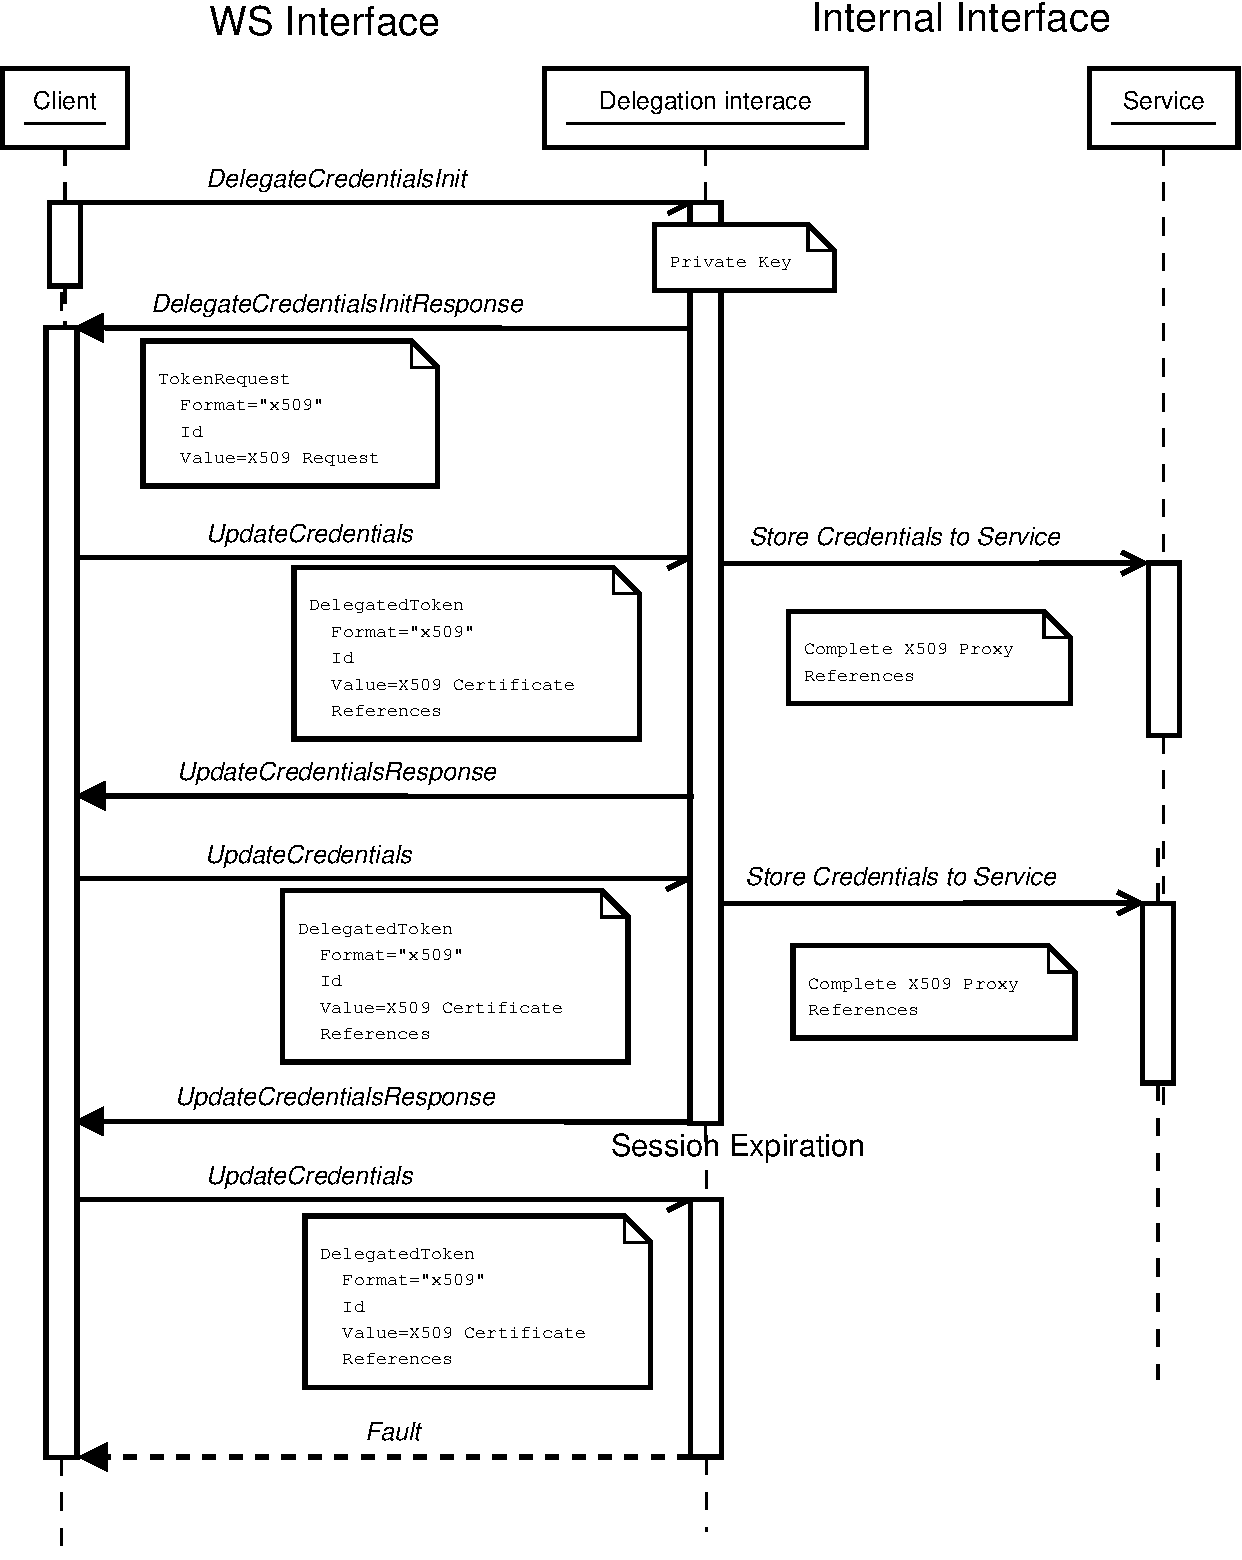
\includegraphics[width=0.9\textwidth]{delegation_flow.pdf}}}
\caption{\label{fig:delegation_flow}The flow diagram of delegation procedure with multiple second step and session expiration} }
\end{figure}

\begin{figure}
\centering{{{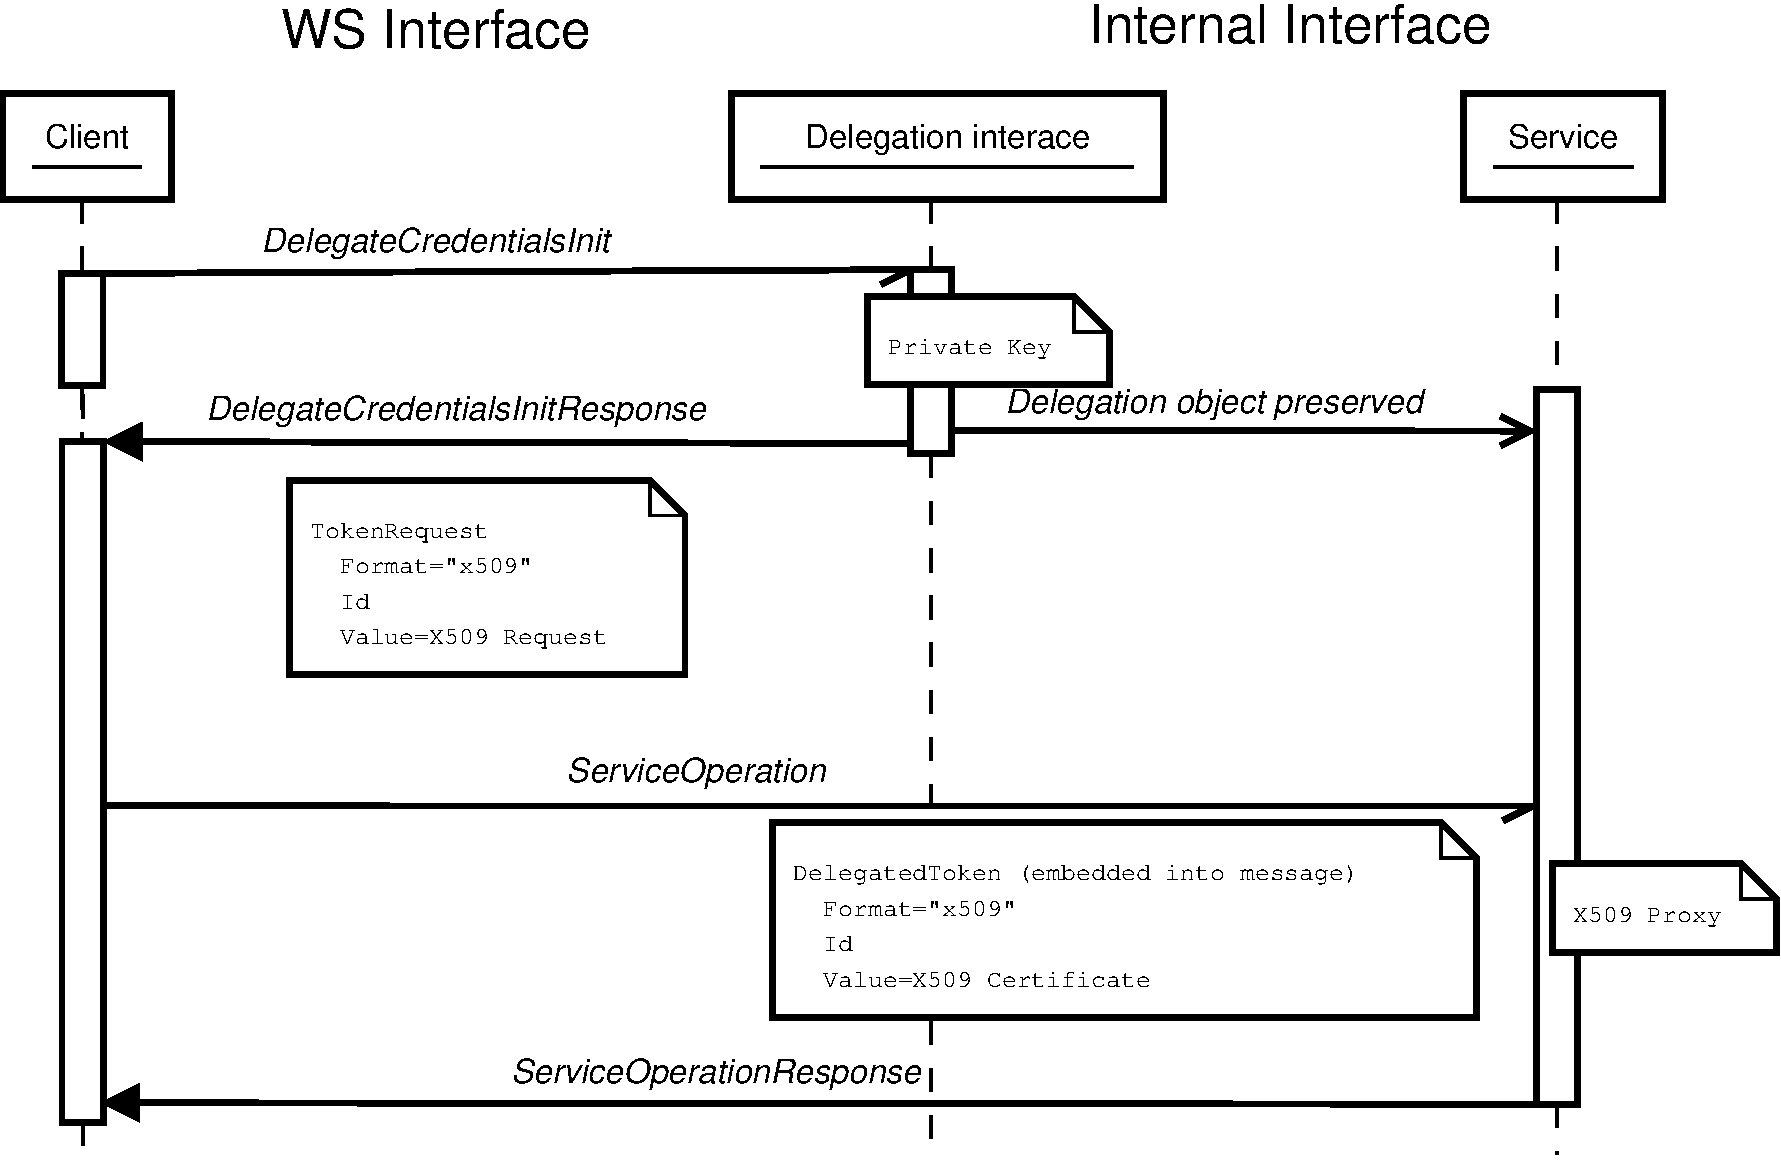
\includegraphics[width=0.9\textwidth]{delegation_flow1.pdf}}}
\caption{\label{fig:delegation_flow1}The flow diagram of delegation procedure with certificate transfered as payload of service specific message} }
\end{figure}

Delegation interface in the ARC NOX is implemented using Web Service approach. Each ARC NOX service wishing to act on behalf of client identity implements this interface in order to accept delegated credentials. Here is how delegation procedure works (also shown in Figure \ref{fig:delegation_flow} and Figure \ref{fig:delegation_flow1}) :

    \begin{itemize}
        \item \emph{Step 1}
            \begin{itemize}
                \item Client contacts service requesting operation DelegateCredentialsInit. This operation has no arguments.
                \item Service responds with DelegateCredentialsInitResponse message with element TokenRequest. That element contains credentials request generated by service in Value. Type of request is defined by attribute Format. Currently only supported format is x509. Along with Value service provides identifier Id which is used in second step.
            \end{itemize}
        \item \emph{Step 2}
            \begin{itemize}
                \item Client requests UpdateCredentials operation with DelegatedToken argument. This element contains Value with serialized delegated credentials and Id which links it to first step. Delegated token element may also contain multiple Reference elements. Reference refers to the object which these credentials should be applied to in a way specific to the service. The DelegatedToken element may also be used for delegating credentials when Step 2 is combined with other operations on service in service specific way.
                \item Service responds with empty UpdateCredentialsResponse message.
            \end{itemize}
    \end{itemize}
Optionally step 2 can be skipped and the DelegatedToken element provided to Service as additional payload of other service specific message.

The Id element obtained in the step 1 can be reused multiple times with different content of the Value element.

WSDL of portType implementing delegation functionality can be found at

http://svn.nordugrid.org/trac/nordugrid/browser/arc1/trunk/src/hed/libs/delegation/delegation.wsdl .


\subsection{Delegated Credentials (Proxy) Generation Utility} % (fold)
\label{subsec:delegation_client}
Command line utility “arcproxy” can be used to generate X.509 Proxy Certificate with (or without)  Policy embedded.
The arcproxy my be used in following way:

\emph{approxy -P proxy.pem -C cert.pem -K key.pem -c constraint}

Here options -P, -C and -K specify path to files containing generated Proxy, user's credentials and user's private key respectively. By using argument ``-c'', some constraints can be specified for proxy certificate. Each constraint string is a key and value pair with key representing type of contraint. There may be multiple -c options specified.  Currently suported contraint types are:

    \begin{itemize}
        \item validityStart, validityEnd and validityPeriod  specify when Proxy becomes valid, when it's validity finishes or for how long the Proxy is valid respectively. For example

-c validityStart=2008-05-29T10:20:30Z

-c validityEnd=2008-06-29T10:20:30Z

        \item proxyPolicy and proxyPolicyFile specify the Policy document to be embedded into the Proxy either directly or by pointing to the file which contains that document. Like

-c proxyPolicyFile=delegation\_policy.xml
    \end{itemize}

The Policy maybe any of any type supported by ARC NOX middleware (or third-party plugins) installed on the services where that policy is processed. Currenlty supported Policies include ARC Policy (described in section \ref{subsec:authz_policy}) and GACL Policy \cite{gacl}.

Simple example below renders delegated credentials usable only for contacting service attached to HTTP communication channel under path /arex (line 5)  and allows HTTP operation POST (line 8) on it.

\begin{verbatim}
1.<?xml version="1.0" encoding="UTF-8"?>
2.<Policy xmlns="http://www.nordugrid.org/schemas/policy-arc" PolicyId="sm-example:policy1"
      CombiningAlg="Deny-Overrides">
3.    <Rule RuleId="rule1" Effect="Permit">
4.        <Resources>
5.            <Resource Type="string"
                  AttributeId="http://www.nordugrid.org/schemas/policy-arc/types/http/path">
                 /arex
              </Resource>
6.        </Resources>
7.        <Actions>
8.            <Action Type="string"
                  AttributeId="http://www.nordugrid.org/schemas/policy-arc/types/http/method">
                  POST
              </Action>
9.        </Actions>
10.   </Rule>
11.</Policy>
\end{verbatim}

Another example of the delegation policy is presented below. This policy restricts usage of delegated credentials to SOAP operation CreateActivity (line 5) of Basic Execution Service (BES) \cite{ogsa-bes} namespace (line 9). Such policy could be embedded into credentials delegated to high level Brokering service performing Grid job submission to low level BES on behalf of user.

\begin{verbatim}
1.<?xml version="1.0" encoding="UTF-8"?>
2.<Policy xmlns="http://www.nordugrid.org/schemas/policy-arc" PolicyId="sm-example:policy1"
    CombiningAlg="Deny-Overrides">
3.    <Rule RuleId="rule1" Effect="Permit">
4.        <Actions>
5.            <Action Type="string"
                AttributeId="http://www.nordugrid.org/schemas/policy-arc/types/soap/operation">
                CreateActivity
              </Action>
6.        </Actions>
7.        <Conditions>
8.            <Condition>
9.                <Attribute Type="string"
                      AttributeId="http://www.nordugrid.org/schemas/policy-arc/types/soap/namespace">
                      http://schemas.ggf.org/bes/2006/08/bes-factory
                  </Attribute>
10.           </Condition>
11.       </Conditions>
12.   </Rule>
13.</Policy>
\end{verbatim}

\subsubsection{Delegated Credentials with VOMS Attributes} % (fold)
\label{subsec:delegation_voms}
Currently the proxy creation utility arcproxy can also be used for creating VOMS Proxy Certificate, as the way to replace the ``voms-proxy-init'' utility.



%section delegation (end)



\section{Web Service Security Support} % (fold)
\label{sec:webservice}

\subsection{UsernameToken SecHandler} % (fold)
\label{subsec:username_token}
The UsernameToken SecHandler is meant for processing - generating and extracting - WS-Security \cite{ws-security} UsernameToken in the SOAP header. Hence it must be attached to the MCC which processes SOAP payloads - like SOAP MCC or Service accepting SOAP messages. For description of configuration see section \ref{subsec:ut_sechandler_conf}.

For the incoming message this SecHandler authorizes SOAP message according to specified configuration.

For the outgoing message this SecHandler creates and adds proper token into SOAP header according to configuration.

\subsection{X509Token SecHandler} % (fold)
\label{subsec:x509_token}
The X.509 Token SecHandler is meant for processing - generating and extracting - WS-Security \cite{ws-security} X.509 Token from SOAP header. Hence it must be attached to the MCC which processes SOAP payloads – like SOAP MCC or Service accepting SOAP messages. For description of configuration see section \ref{subsec:xt_sechandler_conf}.

For the incoming message this SecHandler decrypts and checks signature of SOAP message using attached public key and verifies that key against specified CA certificate.

For the outgoing message this SecHandler creates X.509 Token in SOAP header. SOAP message body is encrypted and signed.

\subsection{SAMLToken SecHandler} % (fold)
\label{subsec:saml_token}
The SAMLToken SecHandler is meant for processing - generating and extracting - WS-Security \cite{ws-security} SAMLToken from SOAP header. Hence it must be attached to the MCC which processes SOAP payloads – like SOAP MCC or Service accepting SOAP messages. For description of configuration see section \ref{subsec:st_sechandler_conf}.

\begin{figure}
\centering{{{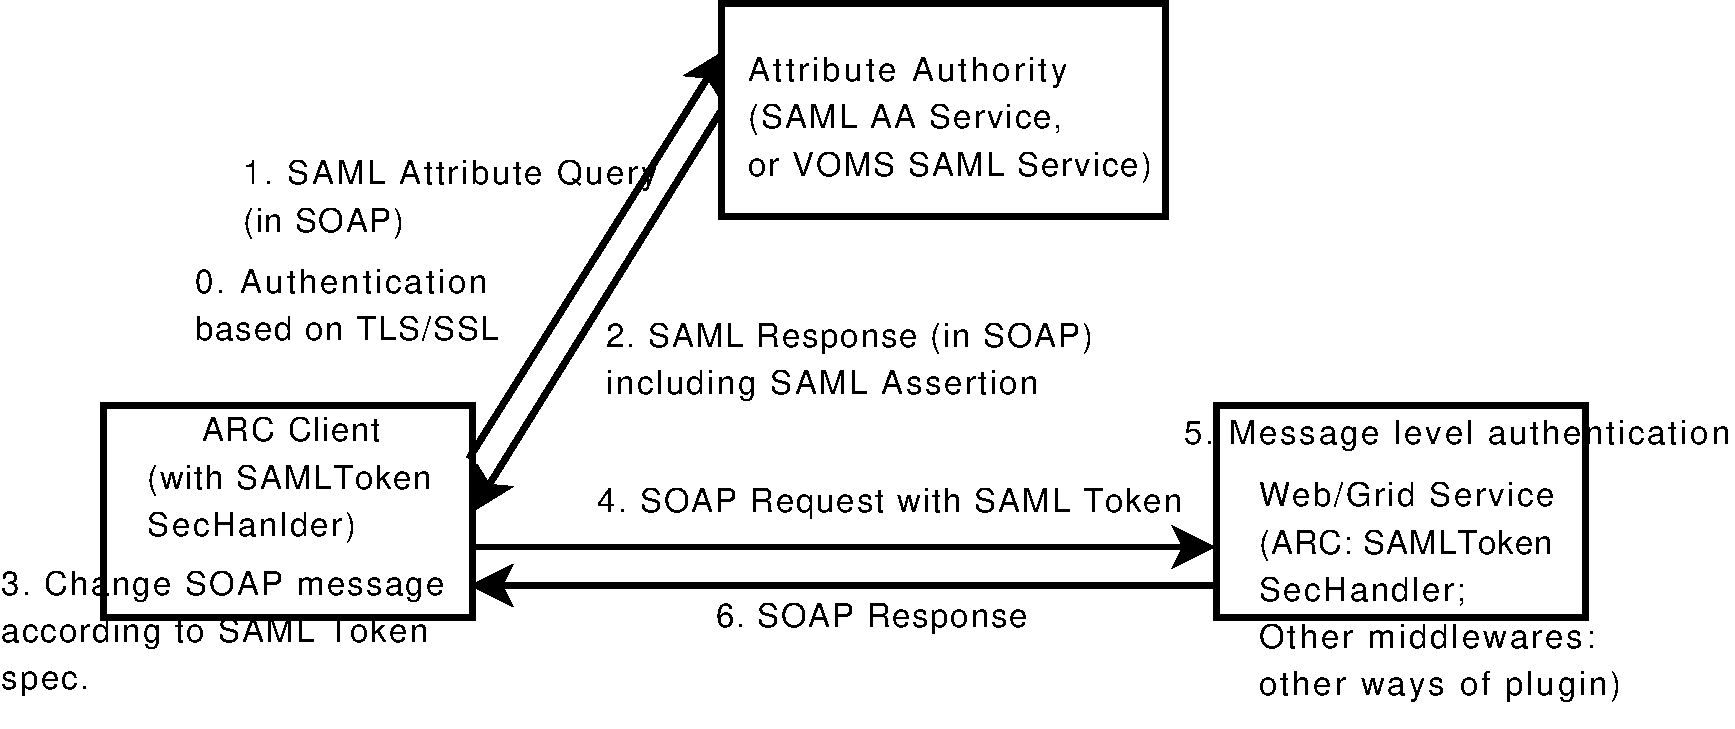
\includegraphics[width=0.9\textwidth]{samltoken_aa.pdf}}}
\caption{\label{fig:samltoken_aa} Interaction among Client, Grid/Web Service and Attribute Authority} }
\end{figure}

Figure \ref{fig:samltoken_aa} shows the interaction among Client, Grid/Web Service and Attribute Authority when SAMLToken security hanlder is deployed. The Attribute Authority service is described in section \ref{sec:saml_aa_service}. For the Grid/Web service, if the service is hosted on ARC middleware, then the SAMLToken security handler should be deployed; if the service is hosted on other middlewares, then there should be other ways for supporting SAML Token authentication, e.g., Rampart (WS-Security modlue for Axis2).

For the incoming message this SecHandler decrypts and checks signature of SOAP message using attached public key and verifies that key against specified CA certificate.

For the outgoing message this SecHandler creates SAMLToken in SOAP header. SOAP message body is encrypted and signed.


%section webservice (end)


\section{Schemas, descriptions and examples} % (fold)
\label{sec:schema_description_example}

\subsection{Authorization Policy} % (fold)
\label{subsec:authz_policy}
XML schema with comments available at

http://svn.nordugrid.org/trac/nordugrid/browser/arc1/trunk/src/hed/shc/arcpdp/Policy.xsd

\subsection{Authorization Request} % (fold)
\label{subsec:authz_request}
XML schema with comments available at

http://svn.nordugrid.org/trac/nordugrid/browser/arc1/trunk/src/hed/shc/arcpdp/Request.xsd


\subsection{Authorization Response} % (fold)
\label{subsec:authz_response}
XML schema with comments available at

http://svn.nordugrid.org/trac/nordugrid/browser/arc1/trunk/src/hed/shc/arcpdp/Response.xsd


\subsection{Interface of policy decision service (Charon service)} % (fold)
\label{subsec:interface_pds}
WSDL with comments available at

http://svn.nordugrid.org/trac/nordugrid/browser/arc1/trunk/src/services/charon/charon.wsdl

The following is the configuration about the Charon service, which is configured to use xacml policy engine. The policy engine is configurable by changing the ``name'' attribute of three elements: \textit{$<$Evaluator$>$}, \textit{$<$Policy$>$}, \textit{$<$Request$>$} into ``arc.evaluator'', ``arc.policy'', ``arc.request''. Also the policy should also be changed to the one with ARC specific format.

\begin{verbatim}
    <Service name="charon" id="charon_service">
        <!--The element <Evaluator/>, <Policy/> and <Request/> configuration
        are supposed to be used to load object; element <PolicyStore/> is
        supposed to be used to get the location of policy-->
        <charon:PDPConfig>
            <charon:PolicyStore>
                <charon:Location Type="file">charon_policy_xacml.xml.example</charon:Location>
                <!-- other policy location-->
            </charon:PolicyStore>
            <charon:Evaluator name="xacml.evaluator" />
            <charon:Policy name="xacml.policy" />
            <charon:Request name="xacml.request" />
        </charon:PDPConfig>
    </Service>
\end{verbatim}

\subsection{TLS MCC configuration} % (fold)
\label{subsec:tlsmcc_conf}
For full description of TLS MCC configuration please read ``The Hosting Environment of the Advanced Resource Connector middleware''. Here only part related to VOMS attributes extraction is provided for convenience. Configuration schema can be found at

http://svn.nordugrid.org/trac/nordugrid/browser/arc1/trunk/src/hed/mcc/tls/tls.xsd

While processing VOMS extension of X.509 certificate only attributes which can be verified are extracted and collected in the list of Security Attributes. To ensure proper authentication trusted VOMS services must to be configured. The VOMS services are identified by certificates which they use to sign AC with VOMS related information. And also by whole certificates chain used to sign VOMS service certificate.

The TLS MCC configuration makes it possible to specify DNs of all certificates in such chains. Each chain is stored in separate \textit{$<$VOMSCertTrustDNChain$>$} element. Each such element is composed either of multiple \textit{$<$VOMSCertTrustDN$>$} elements or single \textit{$<$VOMSCertTrustRegex$>$}

Each \textit{$<$VOMSCertTrustDN$>$} element defined DN of one certificate in a chain starting from certificate of VOMS service and down to DN of last CA in the chain.

The \textit{$<$VOMSCertTrustRegex$>$} element defines regular expression which is applied to every certificate in the chain.

Along with \textit{$<$VOMSCertTrustDNChain$>$} it is also possible to specify \textit{$<$VOMSCertTrustDNChainsLocation$>$}.

The \textit{$<$VOMSCertTrustDNChainsLocation$>$} specifies path to file containing XML document with single \textit{$<$VOMSCertTrustDNChain$>$} element.

Below is an example presenting all possible options.

\begin{verbatim}
<tls:VOMSCertTrustDNChain>
  <tls:VOMSCertTrustDN>/O=Grid/O=NorduGrid/CN=host/arthur.hep.lu.se</tls:VOMSCertTrustDN>
  <tls:VOMSCertTrustDN>/O=Grid/O=NorduGrid/CN=NorduGrid CA</tls:VOMSCertTrustDN>
</tls:VOMSCertTrustDNChain>
<tls:VOMSCertTrustDNChain>
  <tls:VOMSCertTrustDN>/DC=ch/DC=cern/OU=computers/CN=voms.cern.ch</tls:VOMSCertTrustDN>
  <tls:VOMSCertTrustDN>/DC=ch/DC=cern/CN=CERN CA</tls:VOMSCertTrustDN>
</tls:VOMSCertTrustDNChain>
<tls:VOMSCertTrustDNChain>
  <tls:VOMSCertTrustRegex>^/O=Grid/O=NorduGrid</tls:VOMSCertTrustRegex>
</tls:VOMSCertTrustDNChain>
<tls:VOMSCertTrustDNChainsLocation>./voms_trust.xml</tls:VOMSCertTrustDNChainsLocation>
\end{verbatim}


\subsection{Configuration of PDP service} % (fold)
\label{subsec:pdpservice_conf}
XML schema with comments available at

http://svn.nordugrid.org/trac/nordugrid/browser/arc1/trunk/src/services/charon/charon.xsd

Below is an example configuration of PDP service which can evaluate ARC Request against ARC Policy stored in local file.

\begin{verbatim}
<Service name="pdp.service" id="pdp_service">
<!--The element <Evaluator/>, <Policy/> and <Request/> configuration
       are supposed to be used to load object; element <PolicyStore/> is
       supposed to be used to get the location of policy-->
   <pdp:PDPConfig>
       <pdp:PolicyStore>
           <Location Type="file">Policy_Example.xml</Location>
           <!-- other policy location-->
       </pdp:PolicyStore>
       <pdp:Evaluator name="arc.evaluator" />
       <pdp:Policy name="arc.policy" />
       <pdp:Request name="arc.request" />
   </pdp:PDPConfig>
</Service>
\end{verbatim}

See section \ref{subsec:arcpdp_conf} for the explanation of ARC Policy.


\subsection{Authorization SecHandler configuration} % (fold)
\label{subsec:authzhandler_conf}
XML schema with comments available at

http://svn.nordugrid.org/trac/nordugrid/browser/arc1/trunk/src/hed/shc/arcauthzsh/SimpleListAuthZ.xsd

Default behavior of Authorization SecHandler is to execute all PDPs corresponding to elements \textit{$<$PDP$>$} in configuration sequentially till either one of them fails or all produced positive results. This behavior may be modified by attribute ``action'' of embedded \textit{$<$PDP/$>$} elements. Following options are supported:

    \begin{itemize}
        \item breakOnAllow - if PDP returned positive result stop PDPs processing and return positive result. Otherwise continue to next PDP or return negative result if no more PDPs to process. That is a default behavior.
        \item BreakOnDeny - if PDP returned negative result stop PDPs processing and return negative result. Otherwise continue to next PDP or return negative result if no more PDPs to process.
        \item BreakAlways – stop processing PDPs and return result which this PDP returned.
        \item BreakNever – continue to next PDP. If there are no more PDPs to process then return result which this PDP returned.
    \end{itemize}

Below is an example of the Authorization SecHandler with 4 PDPs in the list:

simplelist.pdp – for comparing client's credentilals to list of DNs

arc.pdp – for comparing collected information to specified policies

pdpservice.invoker – for contacting external PDP service.xml

delegation.pdp – for evaluating restrictions embedded into X.509 proxy certificates

\begin{verbatim}
<SecHandler name="arc.authz" id="authz" event="incoming">
  <PDP name="simplelist.pdp" location="simplelistfile"/>
  <PDP name="arc.pdp">
    <PolicyStore>
      <Location type="file">Policy_Example.xml</Location>
    </PolicyStore>
  </PDP>
  <PDP name="pdpservice.invoker">
    <ServiceEndpoint>https://127.0.0.1:60001/pdp.service</ServiceEndpoint>
    <KeyPath>./testkey-nopass.pem</KeyPath>
    <CertificatePath>./testcert.pem</CertificatePath>
    <CACertificatePath>./cacert.pem</CACertificatePath>
  </PDP>
  <PDP name="delegation.pdp"/>
</SecHandler>
\end{verbatim}


\subsection{SimpleList PDP configuration and Policy Example} % (fold)
\label{subsec:simplepdp_conf}
XML schema with comments is available at

http://svn.nordugrid.org/trac/nordugrid/browser/arc1/trunk/src/hed/shc/simplelistpdp/SimpleListPDP.xsd

Below is an example configuration of SimpleList PDP inside ``echo'' service.

\begin{verbatim}
<Service name="echo" id="echo">
  <SecHandler name="arc.authz" id="authz" event="incoming">
    <PDP name="simplelist.pdp" location="simplelist"/>
  </SecHandler>
  <echo:prefix>[ </echo:prefix>
  <echo:suffix> ]</echo:suffix>
</Service>
\end{verbatim}

The attribute ``name'' of \textit{$<$PDP/$>$} is critical for loading the object. Specifically, the name ``simplelist.pdp'' is for loading the SimpleList PDP object.

The policy file ``simplelist'' is a local file which contains the list of X.509 subjects of authorized entities. It the peer certificate is proxy certificate, the identity in this list should only include the original DN of users's certificate.
For example content of simplelist file may look like this:

\emph{/C=NO/O=UiO/CN=test1}

\emph{/C=NO/O=UiO/CN=test2}



\subsection{Arc PDP configuration and Policy Example} % (fold)
\label{subsec:arcpdp_conf}
XML schema with comments available at

http://svn.nordugrid.org/trac/nordugrid/browser/arc1/trunk/src/hed/shc/arcpdp/ArcPDP.xsd

Below is an example of configuration of Arc PDP inside ``echo'' service.
\begin{verbatim}
<Service name="echo" id="echo">
  <SecHandler name="arc.authz" id="authz" event="incoming">
    <PDP name="arc.pdp">
      <PolicyStore>
        <Location type="file">Policy_Example.xml</Location>
        <!--other policy location-->
      </PolicyStore>
    </PDP>
  </SecHandler>
  <echo:prefix>[ </echo:prefix>
  <echo:suffix> ]</echo:suffix>
</Service>
\end{verbatim}

The name ``arc.pdp'' is for loading the ArcPDP object.

There could be a few policy files under \textit{$<$PolicyStore/$>$}. The request will be checked against all of the policies.

There is an example policy for echo service below. See section \ref{subsec:authz_policy} for the policy schema. The example policy is  made of following elements:

  \newcounter{policy_count}
  \begin{list}{\arabic{policy_count}.}
  {\usecounter{policy_count}\setlength{\rightmargin}{\leftmargin}}
    \item Line 14  defines resource being protected. In this it is everything located under HTTP path ``/Echo''.
    \item Lines 17 and 18 define allowed HTTP operations to be ``POST'' and ``GET''. Line 19 also defines SOAP operation ``echo'' to be applied to service at path defined above.
    \item Lines 10 and 9 require the requester to present X.509 certificate with specified identity and signed by specified Certification Authority.
    \item No \textit{$<$Conditions/$>$} defined.
    \item Line 3 defines that if and only if all of the above constraints have been satisfied by requester, the \textit{$<$Rule/$>$} evaluates to Permit decision.
  \end{list}

The Secuirity Attributes used by Arc PDP are collected by different MCCs. It is possible for service to collect some application-specific attributes by implementing class inherited from SecAtt. And that should be the task of application developer.

Administrator of service can configure Authorization SecHandler - arc.authz - for each MCC and Service and define reasonable and meaningful policy. While defining policy the administrator must take into account that the attributes defined in the policy should be already collected by previous components in a chain. For instance, policy with AttributeId ``http://www.nordugrid.org/schemas/policy-arc/types/http/path'' should not be configured inside SecHandler attached to MCCTLS.

\begin{verbatim}
1.<?xml version="1.0" encoding="UTF-8"?>
2.<Policy xmlns="http://www.nordugrid.org/schemas/policy-arc" PolicyId="sm-example:arcpdppolicy"
     CombiningAlg="Deny-Overrides">
3.   <Rule Effect="Permit">
4.     <Description>
5.       Example policy for echo service
6.     </Description>
7.      <Subjects>
8.         <Subject>
9.            <Attribute
               AttributeId="http://www.nordugrid.org/schemas/policy-arc/types/tls/ca"
               Type="string">
               /C=NO/ST=Oslo/O=UiO/CN=CA
              </Attribute>
10.           <Attribute
               AttributeId="http://www.nordugrid.org/schemas/policy-arc/types/tls/identity"
               Type="string">
               /C=NO/ST=Oslo/O=UiO/CN=test
              </Attribute>
11.         </Subject>
12.      </Subjects>
13.      <Resources>
14.         <Resource
             AttributeId="http://www.nordugrid.org/schemas/policy-arc/types/http/path"
             Type="string">
             /Echo
            </Resource>
15.      </Resources>
16.      <Actions>
17.         <Action
             AttributeId="http://www.nordugrid.org/schemas/policy-arc/types/http/method"
             Type="string">
             POST
            </Action>
18.         <Action
             AttributeId="http://www.nordugrid.org/schemas/policy-arc/types/http/method"
             Type="string">
             GET
            </Action>
19.         <Action
             AttributeId="http://www.nordugrid.org/schemas/policy-arc/types/soap/operation"
             Type="string">
             echo
            </Action>
20.      </Actions>
21.      <Conditions/>
22.   </Rule>
23.</Policy>
\end{verbatim}


\subsection{PDP Service Invoker configuration} % (fold)
\label{subsec:pdpservice_invoker_conf}
Configuration XML schema with comments is available at

http://svn.nordugrid.org/trac/nordugrid/browser/arc1/trunk/src/hed/shc/pdpserviceinvoker/PDPServiceInvoker.xsd

Below is an example of configuration of PDP Service Invoker inside ``echo'' service.

\begin{verbatim}
<Service name="echo" id="echo">
  <SecHandler name="arc.authz" id="authz" event="incoming">
    <!--Remote pdp service invoking-->
      <PDP name="pdpservice.invoker">
        <ServiceEndpoint>https://127.0.0.1:60001/pdp.service</ServiceEndpoint>
        <KeyPath>./key.pem</KeyPath>
        <CertificatePath>./cert.pem</CertificatePath>
        <CACertificatePath>./ca.pem</CACertificatePath>
        <RequestFormat>XACML</RequestFormat>
        <TransferProtocol>SAML</TransferProtocol>
      </PDP>
  </SecHandler>
  <next id="echo"/>
  <echo:prefix>[ </echo:prefix>
  <echo:suffix> ]</echo:suffix>
</Service>
\end{verbatim}

The name ``pdpservice.invoker'' defines the PDP Service Invoker object.

The PDP Service Invoker is a client of PDP Service. The configuration options include endpoint of service and credentials to be used for establishing secure connection. In addition, the $<$RequestFormat$>$ element is for specifying the format of the request, and the $<$TransferProtocol$>$ element is for specifying the protocol of tranfering the request.

Table \ref{table:support_pdp_request_protocol} shows the support of request and protocol in remote policy decision making. Note that if ``SAML 2.0 profile of XACML v2.0'' is configured in ``pdpservice invoker'', besides the authorizaton service (called charon service) implemented in ARC, it can interact with external authorization services, such as gLite authorization service (Yet the interoperation test has not been done).

\begin{table}[ht]
\caption{Support of request and protocol in remote policy decision making}
\centering
\begin{tabular}{| l | p{7cm} | p{5cm} |}
\hline
\textbf{  } & \textbf{ARC Request/Response} & \textbf{XACML Request/Response} \\ \hline
\textbf{ARC protocol} & support & support \\ \hline
\textbf{SAML protocol} & not support & support (SAML 2.0 profile of XACML v2.0) \\ \hline
\end{tabular}
\label{table:support_pdp_request_protocol}
\end{table}

\textbf{ARC protocol}:

http://svn.nordugrid.org/trac/nordugrid/browser/arc1/trunk/src/services/charon/charon.wsdl

\textbf{SAML protocol}:

http://svn.nordugrid.org/trac/nordugrid/browser/arc1/trunk/src/services/charon/charon.wsdl

http://www.oasis-open.org/committees/download.php/11475/access\_control-xacml-2.0-saml-protocol-schema-os.xsd

\textbf{ARC request/response}:

http://svn.nordugrid.org/trac/nordugrid/browser/arc1/trunk/src/hed/shc/arcpdp/Request.xsd

http://svn.nordugrid.org/trac/nordugrid/browser/arc1/trunk/src/hed/shc/arcpdp/Response.xsd

\textbf{Note} that the format of ``Response'' is supposed to correspond with the format of ``Request''.

\textbf{XACML request/response}:

http://docs.oasis-open.org/xacml/2.0/access\_control-xacml-2.0-context-schema-os.xsd

http://www.oasis-open.org/committees/download.php/11474/access\_control-xacml-2.0-saml-assertion-schema-os.xsd


\subsection{Delegation PDP configuration} % (fold)
\label{subsec:deleg_pdp_conf}
Configuration XML schema with comments available at

http://svn.nordugrid.org/trac/nordugrid/browser/arc1/trunk/src/hed/shc/delegationpdp/DelegationPDP.xsd

Below is an example of configuration of Delegation PDP inside ``echo'' service.

\begin{verbatim}
<Service name="echo" id="echo">
  <SecHandler name="arc.authz" id="authz" event="incoming">
    <PDP name="delegation.pdp"/>
  </SecHandler>
  <next id="echo"/>
  <echo:prefix>[ </echo:prefix>
  <echo:suffix> ]</echo:suffix>
</Service>
\end{verbatim}

For Delegation PDP, no specific configuration is needed. It is enough to switch it on by adding \textit{$<$PDP name=``delegation.pdp''/$>$} under \textit{$<$SecHandler$>$} which supports processing of PDPs (currently arc.authz).
The precondition for using Delegation PDP is that there must be Delegation SecHandler instantiated earlier in the chain.


\subsection{Delegation SecHandler Configuration} % (fold)
\label{subsec:deleg_sechandler_conf}
Below is an example of configuration of Delegation SecHandler inside TLS MCC component.

\begin{verbatim}
         <Component name="tls.service" id="tls"> <next id="http"/>
            <tls:KeyPath>./key.pem</tls:KeyPath>
            <tls:CertificatePath>./cert.pem</tls:CertificatePath>
            <tls:CACertificatePath>./ca.pem</tls:CACertificatePath>
            <!--delegation.collector must be inside tls MCC-->
            <SecHandler name="delegation.collector"
                id="delegation" event="incoming"></SecHandler>
         </Component>
\end{verbatim}

Current implementation of Delegation SecHandler must be attached to TLS MCC.


\subsection{UsernameToken SecHandler Configuration} % (fold)
\label{subsec:ut_sechandler_conf}
Configuration XML schema with comments is available at

http://svn.nordugrid.org/trac/nordugrid/browser/arc1/trunk/src/hed/shc/usernametokensh/UsernameTokenSH.xsd

Below is an example of configuration of UsernameToken SecHandler inside MCCSOAP component of the service side. This example processes UsernameToken related information in SOAP message and returns failure if any problem found. In detail, this SecHandler will check header of the incoming SOAP message for the presence of UserName WS-Security token and compare provided password value to those stored in the local file password.txt.

\begin{verbatim}
<Component name="soap.service" id="soap">
  <next id="echo"/>
  <SecHandler name="usernametoken.handler" id="usernametoken" event="incoming">
    <Process>extract</Process>
    <PasswordSource>password.txt</PasswordSource>
  </SecHandler>
</Component>
\end{verbatim}

This example will add token with username ``user'' and password ``pass'' (using ``digest'' encoding algorithm) into outgoing SOAP message.

For the client side, the developer should add the configuration information about X.509 security handler into client's configuration, in order to generate X.509 Token into any SOAP message. Below is an example of how to use it:

\begin{verbatim}
    Arc::XMLNode sechanlder_nd_ut("\
        <SecHandler name='usernametoken.handler' id='usernametoken' event='outgoing'>\
            <Process>generate</Process>\
            <PasswordEncoding>digest</PasswordEncoding>\
            <Username>user</Username>\
            <Password>passwd</Password>\
        </SecHandler>");
  Arc::ClientSOAP *client;
  client = new Arc::ClientSOAP(mcc_cfg,url);
  client->AddSecHandler(sechanlder_nd_ut, "arcshc");
\end{verbatim}

\subsection{X509Token SecHandler configuration} % (fold)
\label{subsec:xt_sechandler_conf}
Configuration XML schema with comments is available at

http://svn.nordugrid.org/trac/nordugrid/browser/arc1/trunk/src/hed/shc/x509tokensh/X509TokenSH.xsd

Below is an example of configuration of X.509 Token SecHandler inside MCCSOAP component of the service side. This example processes X.509 Token related information in SOAP message and returns failure if any problem found.

\begin{verbatim}
<Component name="soap.service" id="soap">
  <next id="echo"/>
  <SecHandler name="x509token.handler" id="x509token" event="incoming">
    <Process>extract</Process>
    <CACertificatePath>ca.pem</CACertificatePath>
  </SecHandler>
</Component>
\end{verbatim}

For the client side, the developer should add the configuration information about X.509 security handler into client's configuration, in order to generate X.509 Token into any SOAP message. Below is an example of how to use it:

\begin{verbatim}
  Arc::XMLNode sechanlder_nd_xt("\
        <SecHandler name='x509token.handler' id='x509token' event='outgoing'>\
            <Process>generate</Process>\
            <CertificatePath>./testcert.pem</CertificatePath>\
            <KeyPath>./testkey-nopass.pem</KeyPath>\
        </SecHandler>");
  Arc::ClientSOAP *client;
  client = new Arc::ClientSOAP(mcc_cfg,url);
  client->AddSecHandler(sechanlder_nd_xt, "arcshc");
\end{verbatim}


\subsection{SAMLToken SecHandler Configuration} % (fold)
\label{subsec:st_sechandler_conf}
Configuration XML schema with comments is available at

http://svn.nordugrid.org/trac/nordugrid/browser/arc1/trunk/src/hed/shc/samltokensh/SAMLTokenSH.xsd

%section schema_description_example (end)


\section{Using SAML2 Web SSO for Authentication and Attribute-based Authorization} % (fold)
\label{sec:samlsso}
   In ARC NOX, besides that GSI is supported for talking with external Grid services which are based on GSI, the standard TLS/SSL is also supported. No matter standard SSL/TLS or GSI is used, mutual authentication applies for both of them, and is the default configuration for Grid deployment; and X.509 certificate is required for both of the client and service sides. X.509 certificates is issued by certificate authorities (CA), and then CAs constitute trust federation and guarantee two different X.509 certificates from different CAs can accomplish authentication to each other. So if a user would access Grid system, he/she should own a X.509 certificate which is issued by a CA that is trusted by other's entity in the Grid system.

   ARC NOX provides another option by which users are not required to possess a X.509 certificate for authentication. It is based on AAI(Authentication and Authorization Infrastructure) and utilize users' existing community credential (such as username password) for authentication rather than X.509 credential.

   SAML 2.0 specification defines the Web browser SSO profile which is a standardization for single sign-on (SSO). SSO enables the establishment of federated environment in which clients can sign in the home organization once and access services offered by different external organizations. By using SAML2.0 Web browser SSO profile, users can access external organizations by only authenticating to their own organization. Also instead of requiring users to possess X.509 credential, different authentication mechanisms, such as username/password authentication, IP address authentication, etc.

  The essential idea of SAML2.0 Web browser SSO profile is that uses can access external resources by only depending on their own existing credentials, instead of applying a new credential for accessing external organization. Concerning the use case of Grids which commonly require users to obtain a X.509 credential for the access to Grid, even if these users already have possessed the credential from their host organizations, integrating SAML2.0 SSO profile into Grid usage is considered to be a promising direction for the widely take up of Grids. The SAML2.0 web browser SSO profile is implemented in ARC middleware as another option for authentication, beside the mutual SSL/TLS authentication.

  SAML2.0 SSO profile defines three functional components, an Identity Provider, a Service Provider, and a user agent. The Identity Provider (IdP) is responsible for creating, maintaining, and managing user identity.  The Service Provider (SP) is responsible for controlling access to services and resources by using the SAML assertion produced and issued by IdP upon request. The user agent is responsible for initiating the access request to SP and redirecting the message between SP and IdP, and user agent is commonly hosted inside Web browser. There are several implementations of SAML2.0 SSO profile, among which Shibboleth is one implementation which has been widely deployed.

    In terms of implementation, since the SSO profile is primarily supposed to protect Web applications and provide authentication for Web users, some external code on the client and service side is implemented to integrate the SSO profile. On the client side, apart from the client interface for writing Web Service client, the user agent functionality of the Web browser is implemented in order to mimic its behavior, such as HTTP redirection and HTTP cookie processing. In fact, implementation of the user agent is also based on the client interface of ARC, specifically, the HTTPs client interface, since the client interface of ARC can support different protocols which are incarnated by different MCCs. The client developers who would use SAML2.0 SSO profile should call the user agent interface and then the Web Service client interface. On the service side, the Service Provider functionality (based on the HTTP MCC configured together with TLS MCC) is implemented by SP Service. For Identity Provider, the Shibboleth IdP implementation is used. Figure 8 shows the process of SAML2.0 SSO integrated in ARC client and service.

   Normally SP service will not be deployed independently, instead, it should be deployed together with other services. The SLCS service is the typical deployment about SP service. On the client side, client developer should use the ClientSAML2SSO instead of ClientInterface to call the client functionality. The SLCS client (arcslcs) is the typical usage of  ClientSAML2SSO interface.

    Once the SP Service has cooperated with user agent and Identity Provider (external) and succeeded to accomplish the SAML2 SSO profile,  the SP service will get the saml authentication assertion which asserts that the authentication has succeeded, and then SP service will store this assertion into session context.

    SAML2 assertion consumer handler (saml2ssoassertionconsumer.handler) is the security handler which will understand the authentication assertion and attribute assertion from IdP, and make authorization decision according to the attribute values inside these assertions. Currently the SAML2 assertion consumer handler is an empty security handler and does not effect the services.


The steps shows in Figure 8 are described as follows:

  \newcounter{sso_count}
  \begin{list}{\arabic{sso_count}.}
  {\usecounter{sso_count}\setlength{\rightmargin}{\leftmargin}}
    \item The client uses the user agent interface to launch a HTTP request including the IdP name (to which the user belongs) to the service side. The endpoint of the SP (Service Provider) service is the same as that of the other target services, except the last part of the endpoint is ``saml2sp'' which is specific for pointing to the SP Service. Note that we use Identity Provider (IdP) name here to simplify the IdP discovery process in order to avoid the IdP discovery process, because we suppose that the user who would access the target services should better know where is he from initially.

    \item The SP Service searches the metadata (we use the same metadata format as defined in Shibboleth) and gets the location of the single sign-on service (hosted in IdP) and also the location of assertion consuming service (hosted in this SP itself) in order to compose the SAML $<$samlp:AuthnRequest$>$ message. Then SP Service issues this $<$samlp:AuthnRequest$>$ message by using its own X.509 certificate (note that in the SAML SSO profile, X.509 certificates are still needed for IdP and SP) and sends back to user agent.

    \item User agent sends the $<$samlp:AuthnRequest$>$ message to the Identity Provider.

    \item Identity Provider requires an act of authentication. The authentication mechanism is outside of the SAML2.0 SSO profile. Shibboleth IdP implementation chooses some login handlers for authentication. The current user agent implementation is compatible with the Username/Password login handler of Shibboleth IdP. Through the HTTP protocol, the user agent will feed IdP with the username/password which has been given by the caller of user agent interface.

    \item Once the authentication has been succeeded, the IdP issues a SAML response including an encrypted (encrypted by destination SP’s public key) SAML assertion, and then this SAML response will be delivered by the user agent to the Service Provider.

    \item The SP Service verifies and checks the SAML response, decrypts and stores the SAML assertion into session/connection context. The SAML assertion includes the $<$saml:AuthnStatement$>$ and $<$saml:AttributeStatement$>$.

    \item The WS client launches the Grid/Web Service request via the same connection as the one which is used by user agent to contact SP Service.

    \item The Grid/Web Service checks the $<$saml:AuthnStatement$>$ from the session context to see if the session is still valid through the SecHandler called ``SAML assertion consumer SecHandler''. If valid, service handles the service processing and returns the response to WS client. Note that service requires that WS client is from the same connection as the one on which user agent contact SP service, in order to guarantee that the validity of SSO profile result effects the WS client/Web Service interaction.

    The SP service and other functional service(s) are hosted by the same container, and they use the same X.509 credential. The client authentication is switched off, so that client doesn’t need to use any X.509 credential. Only the trusted certificates (CA certificates for both SP and IdP) need to be configured for the client side, so that SP and IdP can authenticate themselves to the client. As required by the SAML2.0 profile, the SP and IdP should have trust relationship to each other.
   \end{list}

    A typical configuration for service that is enhanced by SAML2SSO profile is as follows:

\begin{verbatim}
    <Chain>
        <Component name="tcp.service" id="tcp">
            <next id="tls"/>
            <tcp:Listen><tcp:Port>60000</tcp:Port></tcp:Listen>
        </Component>
        <Component name="tls.service" id="tls">
            <next id="http"/>
            <tls:KeyPath>./testkey-nopass.pem</tls:KeyPath>
            <tls:CertificatePath>./testcert.pem</tls:CertificatePath>
           <!--Since the client side's certificate is not required to exist,
            the trusted CA certificates are not needed here-->
            <!--tls:CACertificatePath>./cacert.pem</tls:CACertificatePath-->
           <!--Client side authentication is not required-->
            <tls:ClientAuthn>false</tls:ClientAuthn>
        </Component>
        <Component name="http.service" id="http">
            <next id="plexer">POST</next>
        </Component>
        <Plexer name="plexer.service" id="plexer">
            <next id="samlsp">/saml2sp</next>
            <next id="soap">/echo</next>
            <!--Other services ID can be put here-->
            <!--next id="soap">/aotherservice</next-->
        </Plexer>
        <Component name="soap.service" id="soap">
            <next id="echo"/>
           <!--The security handler used for doing, e.g., access control based on
           the SAML assertion from the SAML2.0 SSO profile; currently it is just a
            prototype implementation-->
            <SecHandler name="saml2ssoassertionconsumer.handler" id="saml2ssosp" event="incoming"/>
        </Component>
        <Service name='saml.sp' id='samlsp'>
            <!--Metadata that is according to SAML metadata standard.
             urn:oasis:names:tc:SAML:2.0:metadata-->
            <MetaDataLocation>./test_metadata.xml</MetaDataLocation>
            <!--The entity ID of this Service Provider-->
            <ServiceProviderName>https://squark.uio.no/shibboleth-sp</ServiceProviderName>
            <!--The certificate and key file which will be used by Service Provide
             to sign the AuthnRequest-->
            <KeyPath>./testkey-nopass.pem</KeyPath>
            <CertificatePath>./testcert.pem</CertificatePath>
        </Service>
        <Service name="echo" id="echo">
            <next id="echo"/>
            <echo:prefix>[ </echo:prefix>
            <echo:suffix> ]</echo:suffix>
        </Service>
    </Chain>
\end{verbatim}

    The client developer should use the ClientSOAPwithSAML2SSO  or ClientHTTPwithSAML2SSO instead of ClientInterface for the integration of SAML2SSO profile. A typical usage of ClientSOAPwithSAML2SSO is shown as follows. Note the IdP name and the username/password should be feed as the input argument for ``process'' method.

\begin{verbatim}
   Arc::ClientSOAPwithSAML2SSO *client = NULL;
   client = new Arc::ClientSOAPwithSAML2SSO(mcc_cfg,url);
   Arc::MCC_Status status = client->process(&req,&resp, idp_name, username, password);
\end{verbatim}

    The message flow of interaction between Client, ARC SP Service, ARC Service and Shibboleth IdP is also shown in Figure.9.

  One benefit of the SAML2.0 SSO profile that is worth mentioning is: the Identity Provider could cache the authentication result through session management once the user agent has succeeded to authenticate; then for a short period this authentication result is valid so that the user agent doesn’t need to feed IdP with user’s username and password the next time (if this point of time is not out of the scope of valid period) it authenticates against IdP. So user (or the client on behalf of this user) can access multiple security  domains with only providing his name and password once, which is the characteristic of single sign-on.

    Since the Shibboleth implementation of SAML is standard-compliant and widely deployed, the solution implemented in ARC can easily interoperate with other SAML implementations with minimum change, and more importantly, this solution can succeed to utilize the widely deployed SAML implementation for authentication in Grid systems by avoiding the usage of X.509 certificate.


%section samlsso (end)


\section{Short-Lived Credential Service} % (fold)
\label{sec:slcs}
In order to create X.509 credential for inter-operating with Grid services that requires client side certificate authentication, based on the solution described in section \ref{sec:samlsso}, a short lived credential service (SLCS) is implemented by which user can get a short-lived X.509 certificate without being bothered to contact any registration authority (RA) or certificate authority (CA).

    SLCS service is for signing short-lived x509 credential based on user's username/password credential. Then the user can use this short-lived x509 credential to access Grid services/resources where x509 credential is required by default. SLCS service should depend on the SP (Service provider) service which is one of the participants of SAML2 SSO profile (SAML2 SSO profile is used for authenticating based on username/password credential and getting SAML authentication assertion; and SAML authentication assertion is then used as basis for signing short-lived x509 credential).

    The SLCS service is also a Web Service (standard Web Service implemented by using ARC service interface), and the SLCS client is a specific command-line interface (CLI) which includes the user agent and WS client. The whole process of SLCS invocation is showed in Figure 10 (from step 1 to step 8), which is the same as in Figure 8, except that step 7 and step 8 are invoked for the SLCS certificate request and response.


 SLCS service is supposed to run together with SP service. A typical configuration for SLCS service is as follows:

\begin{verbatim}
    <Chain>
        <Component name="tcp.service" id="tcp">
            <next id="tls"/>
            <tcp:Listen><tcp:Port>60000</tcp:Port></tcp:Listen>
        </Component>
        <Component name="tls.service" id="tls">
            <next id="http"/>
            <tls:KeyPath>./testkey-nopass.pem</tls:KeyPath>
            <tls:CertificatePath>./testcert.pem</tls:CertificatePath>
            <!--tls:CACertificatePath>./cacert.pem</tls:CACertificatePath-->
            <tls:ClientAuthn>false</tls:ClientAuthn>
        </Component>
        <Component name="http.service" id="http">
            <next id="plexer">POST</next>
        </Component>
        <Plexer name="plexer.service" id="plexer">
            <next id="samlsp">/saml2sp</next>
            <next id="soap">/slcs</next>
        </Plexer>
        <Component name="soap.service" id="soap">
            <next id="slcs"/>
            <SecHandler name="saml2ssoassertionconsumer.handler" id="saml2ssosp" event="incoming"/>
        </Component>
        <Service name='saml.sp' id='samlsp'>
            <MetaDataLocation>./test_metadata.xml</MetaDataLocation>
            <ServiceProviderName>https://squark.uio.no/shibboleth-sp</ServiceProviderName>
            <KeyPath>./testkey-nopass.pem</KeyPath>
            <CertificatePath>./testcert.pem</CertificatePath>
        </Service>
        <Service name="slcs.service" id="slcs">
            <next id="slcs"/>
            <slcs:CACertificate>./CAcert.pem</slcs:CACertificate>
            <slcs:CAKey>./CAkey.pem</slcs:CAKey>
            <slcs:CASerial>./CAserial</slcs:CASerial>
        </Service>
    </Chain>
\end{verbatim}

    SLCS service and SP service should together be configured by using the Plexer. SP service is directly based on http and SLCS is directly based on soap. As shown in the above table, a plexer dispatches the message flow (outgoing from http.service) into two SP service (saml.sp) and SOAP service (soap.service).

    Since the client authentication is switched off, it is not necessary to configure $<$CACertificatePath$>$ or $<$CACertificateDir$>$ for TLS MCC.

    SP service needs to be configured with $<$MetaDataLocation$>$ and $<$ServiceProviderName$>$.

    SLCS service should specifically include the CA credential (certificate and key file) and the serial number file (which includes the serial number of each signed certificate), so SLCS service needs to be configured with $<$CACertificate$>$ $<$CAKey$>$ and $<$CASerial$>$. Therefore, the service administrator should firstly create a CA credential (note for interoperability purpose in the production Grid deployment, the CA credential should be trusted by others).

Note: When deploying the SLCS service, service administrator should deploy a dedicated IdP (Identity Provider) which can be assigned as authentication/attribute authority, or the users should have already had his own IdP. And the IdP information (authentication URL and attribute authority URL) should have already been included into the metadata of above configuration (e.g. test\_metadata.xml). On the other hand, the SP (SP service) information (assertion consuming URL) should also have been included into the metadata of the IdP.

    After the whole process, user only needs to authentication with his existing IdP and can get back the x509 credential.

    Shibboleth IdP (http://shibboleth.internet2.edu) is used for the current solution of IdP, since it is widely deployed for other AAI (Authentication and Authority Infrastructure). There is a test IdP deployed in https://squark.uio.no:8443 (idpname: https://squark.uio.no/idp/shibboleth, username: staff, password: 123456), you can use the SP from https://sp.testshib.org/ to test the validity of the test IdP. And also you can installed your own IdP which is supposed to authenticates the users from your own organization.

    SLCS client generates  a X.509 certificate  request, launches a Web Service request which includes the certificate request; SLCS service then gets the certificate request, composes a distinguished name (DN), issues a certificate (short lived, 12 hours by default) with the SAML attribute (from the SAML2.0 SSO profile) as the X.509 certificate extension, and puts the certificate in to the Web Service response; SLCS client get the response and stores the X.509 certificate into local repository.

The CLI for the SLCS client is like this:

\textit{./arcslcs -S https://127.0.0.1:60000/slcs -I https://idp.testshib.org/idp/shibboleth -U myself -P myself}

    Since the lifetime of the short lived credential is normally short, it is not a must to protect the private key by a pass phrase. As illustrated in steps (a) and (b) in Figure 10, if the private key is not protected through the Web Service client, the user can use the X.509 certificate to access Grid Service or Web Service from any kind of middleware. If the private key is protected, she can use the X.509 certificate to generate a proxy certificate (by using a command-line interface utility such as grid-proxy-init , voms-proxy-init, or arcproxy ), and then use the proxy certificate to access a Grid/Web Service.

    Composing the distinguished name (DN) for the certificate is a critical issue for the SLCS service. Since the Shibboleth Identity Provider uses the eduPerson schema for the definition of $<$saml:Attribute$>$ in $<$saml:AttributeStatement$>$, we pick the relatively distinguishable attribute \textit{``eduPersonPrincipalName''} for the DN. A typical eduPersonPrincipalName value could be \textit{alice@example.org}, then the DN is

\textit{``/O=knowarc/OU=example.org/CN=alice''}.

    The obvious benefit of the SLCS service is that: If a user passes the authentication to her home Identity Provider, she can get the X.509 credential anywhere simply by running the SLCS client command together with providing her username and password to this home IdP, and then access the Grid system conveniently.

\subsection{The Usage of SLCS client} % (fold)
\label{subsec:slcs_client}

    On the SLCS client side, there is a client utility called ``arcslcs''.  The command option for arcslcs is as following:
Application Options:

  -S, --url=url                URL of SLCS service

  -I, --idp=string             IdP name

  -U, --user=string            User account to IdP

  -P, --password=string        Password for user account to IdP

  -Z, --keysize=number         Key size of the private key (512, 1024, 2048)

  -K, --keypass=passphrase     Private key passphrase

  -L, --lifetime=period        Lifetime of the certificate, start with current time, hour as unit

  -D, --storedir=directory     Store directory for key and signed certificate

  -z, --conffile=filename      configuration file (default ~/.arc/client.conf)

An example is:

\textit{./arcslcs -S https://127.0.0.1:60000/slcs -I https://squark.uio.no/idp/shibboleth -U root -P aa1122 -D   ~/arc-0.9/src/clients/credentials -z client.confg}

    Note user should input the ``IdP name'' is the corresponding Identity Provider (one of the participants of SAML2 SSO profile) name to which the user would authenticate against by using its username/password credential. And the name is stored inside the metadata on both SP service and IdP provider, and it is used by SP service to get the authentication URL for username/password based authentication.

    And the ``user'' and ``password'' is the credential which will be used to authentication against IdP.
The ``conffile'' can be another option for all of the above options, see the following as an example:

\begin{verbatim}
[common]
keypath=./testkey-nopass.pem
certificatepath=./testcert.pem
cacertificatesdirectory=./certificates
slcsurl=https://127.0.0.1:60000/slcs
idpname=https://squark.uio.no/idp/shibboleth
username=root
password=aa1122
keysize=1024
keypass=123456
certlifetime=24
storedir=./
verbosity=INFO
\end{verbatim}

    There is a temporary Identity Provider (IdP) deployed on squark.uio.no for test with the following test username and password: staff, researcher, librarian, binduser ; with the same password ``123456''

\textit{./arcslcs -S https://127.0.0.1:60000/slcs -I https://squark.uio.no/idp/shibboleth -U staff -P 123456 -D /home/wzqiang/arc-0.9/src/clients/credentials -z client.conf}

    The short-lived credential issued by SLCS service will include the SAML assertion as the extension of X.509 certificate as a proof of passing SAML2 SSO profile.



%section slcs (end)


\section{X.509 Credential Delegation Service} % (fold)
\label{sec:delegation_service}
Besides the delegation interface described in section \ref{subsec:delegation_interface}, which provides interface for X.509 credential delegation. A dedicated Web Service is also developed for credential delegation, with the intention of providing a general approach for using delegation by changing the configuration information, rather than a specific approach which requires directly changing the code.

    As shown in Figure 11, there is a specific WS client and Web Service for processing delegation: delegation client, and delegation service. The WSDL (Web Service Description Language) of the delegation service has three main operations, the first one for processing the delegation initiation, the second one for storing the signed proxy certificate, and the last one for processing acquisition of the delegated credential. The sequential diagram of the delegation is detailed in Figure 12.

    For the delegation process, the delegation WS client functionality (inside each delegation service or the initial client) which is included to access the target delegation service (d1 or d2 in Figure 11), should use the user’s X.509 credential or a delegated credential (on behalf of the user) for authentication and secure communication, as well as delegate one more level of the delegated credential. For the other general  service invocation process, the WS client functionality (inside each service or the initial client) which is included to access the target service (step a1 or a2 in Figure 11), should also use the user’s X.509 credential or a delegated credential for authentication and secure communication.

    Since each WS client accesses the target service (delegation service or other general services) on behalf of the user, the trust relationship between the user’s certificates (X.509 certificate and proxy certificate) and services is required, while the trust relationship between service’s certificate and another service’s certificate is not required.

Below is the configuration of the delegation service, and the ``echo'' service which contacts the delegation service to acquire the delegated certificate.

The configuration of the delegation service which is located at ``glueball.uio.no''.

\begin{verbatim}
    <Chain>
        <Component name="tcp.service" id="tcp">
            <next id="tls"/>
            <tcp:Listen><tcp:Port>60005</tcp:Port></tcp:Listen>
        </Component>
        <Component name="tls.service" id="tls">
            <next id="http"/>
            <tls:KeyPath>./testkey-nopass.pem</tls:KeyPath>
            <tls:CertificatePath>./testcert.pem</tls:CertificatePath>
            <tls:CACertificatePath>./cacert.pem</tls:CACertificatePath>
              <tls:CACertificatesDir>./certificates</tls:CACertificatesDir>
        </Component>
        <Component name="http.service" id="http">
            <next id="soap">POST</next>
        </Component>
        <Component name="soap.service" id="soap">
            <next id="delegation"/>
        </Component>
        <Service name="delegation.service" id="delegation">
            <next id="delegation"/>
            <deleg:CACertificatesDir>./certificates</deleg:CACertificatesDir>
            <deleg:CACertificatePath>./testcacert.pem</deleg:CACertificatePath>
        </Service>
    </Chain>
\end{verbatim}

The configuration of the ``echo'' service (e.g., located at ``selectron.uio.no'') which contacts the delegation service that is located at ``glueball.uio.no''.

\begin{verbatim}
    <Chain>
        <Component name="tcp.service" id="tcp">
            <next id="tls"/>
            <tcp:Listen><tcp:Port>60000</tcp:Port></tcp:Listen>
        </Component>
        <Component name="tls.service" id="tls">
            <next id="http"/>
            <tls:KeyPath>./testkey-nopass.pem</tls:KeyPath>
            <tls:CertificatePath>./testcert.pem</tls:CertificatePath>
            <tls:CACertificatePath>./cacert.pem</tls:CACertificatePath>
              <tls:CACertificatesDir>./certificates</tls:CACertificatesDir>
        </Component>
        <Component name="http.service" id="http">
            <next id="soap">POST</next>
        </Component>
        <Component name="soap.service" id="soap">
            <next id="echo"/>
        </Component>
        <Service name="echo" id="echo">
            <SecHandler name='delegation.handler' id='delegation' event='incoming'>
              <deleg:Type>x509</deleg:Type>
              <deleg:Role>delegatee</deleg:Role>
              <deleg:DelegationServiceEndpoint>
                https://glueball.uio.no:60000/delegation
              </deleg:DelegationServiceEndpoint>
              <!--The credential and trusted certificates which will be used by this
              security handler to contact with delegation service -->
              <deleg:KeyPath>./testkey-nopass.pem</deleg:KeyPath>
              <deleg:CertificatePath>./testcert.pem</deleg:CertificatePath>
              <deleg:CACertificatesDir>./certificates</deleg:CACertificatesDir>
              <deleg:CACertificatePath>./testcacert.pem</deleg:CACertificatePath>
            </SecHandler>
            <next id="echo"/>
            <echo:prefix>[ </echo:prefix>
            <echo:suffix> ]</echo:suffix>
        </Service>
    </Chain>
\end{verbatim}

On the client side of ``echo'' service, the client developer is supposed to add the following piece of configuration into the client configuration information, by adding one line of code:

\begin{verbatim}
client->AddSecHandler(sechanlder_nd, "arcshc");
\end{verbatim}

Some explanation about the configuration is described.

\begin{verbatim}
     Arc::XMLNode sechanlder_nd("\
        <SecHandler name='delegation.handler' id='delegation' event='outgoing'>\
          <Type>x509</Type>\
          <Role>delegator</Role>\
          <!--The endpoint of delegation service, to which this security handler will
          delegate the credential-->\
          <DelegationServiceEndpoint>\
            https://glueball.uio.no:60005/delegation
          </DelegationServiceEndpoint>\
          <!--The endpoint of the peer service, to which this WS client will access-->\
          <PeerServiceEndpoint>https://selectron.uio.no:60000/echo</PeerServiceEndpoint>\
         <!--The key and certificate of the credential, which is be delegated to the
         delegation service-->\
          <KeyPath>./testkey-nopass.pem</KeyPath>\
          <CertificatePath>./testcert.pem</CertificatePath>\
         <!--Another option of defining the location of credential-->\
          <!--ProxyPath>/tmp/5612d050.pem</ProxyPath-->\
         <!--Yet another option of defining how to get the credential; this option is
         useful for the service which has already acquired the delegated credential
         (this delegated credential is stored under /tmp/hash_value.pem) from the
         delegation service, yet still needs to delegate this credential to another delegation
         service; the DelegationCredentialIdentity can be parsed from the tls connection from
         client side, and then used to calculate the hash value to get the delegated credential
         from local repository-->\
          <!--DelegationCredIdentity>/O=KnowARC/OU=UiO/CN=squark.uio.no</DelegationCredIdentity-->\
          <CACertificatePath>./cacert.pem</CACertificatePath>\
          <CACertificatesDir>./certificates</CACertificatesDir>\
        </SecHandler>");
\end{verbatim}


%section delegation_service (end)


\section{SAML Attribute Authority Service} % (fold)
\label{sec:saml_aa_service}
SAML Attribute Authority Service (SAML AA Service) is implemented for accepting SAML \textit{$<$samlp:AttributeQuery$>$} from the requester, and issuing SAML \textit{$<$samlp:Response$>$} which is supposed to include \textit{$<$saml:Assertion$>$} that contains the attribute information about the requester. The implementation is according to the SAML 2.0 ``Assertion Query/Request Profile'', see paragraph 6 of the ``Profiles for the OASIS Security Assertion Markup Language (SAML) V2.0'':

http://docs.oasis-open.org/security/saml/v2.0/saml-profiles-2.0-os.pdf

SAML AA service is implemented with the same functionality as VOMS SAML service. More specifically, the interface of SAML AA service is the same as VOMS SAML service.

The client functionality of \textbf{SAML AA service} exists in two places:

\begin{itemize}
    \item The specific client utility (saml\_assertion\_init), where the SAML AA service is contacted to get back the SAML assertion; Also it is planned to put this client functionality into the client utility ``arcproxy'', so that the the returned SAML assertion will be one of the \textit{``extentions''} of proxy certificate.

    \item The security handler about SAML token, where the SAML AA service is contacted and then the responded SAML assertion is inserted into SOAP message according to WS-Security SAML Token profile.

\end{itemize}

As a way of managing the attributes related to the requesters, the VOMS Admin service is used. Also the database schema that is used in VOMS is also introduced into ARC.

Therefore, the following packages about VOMS Admin service are currently required for the running of SAML AA Service:

glite-security-voms-admin-server-2.0.15-1

glite-security-voms-admin-interface-2.0.2-1

glite-security-voms-admin-client-2.0.8-1

\textit{Note} that the version of these pakages could be updated according to the updating of gLite middlware.

\begin{figure}[ht]
\centering{{{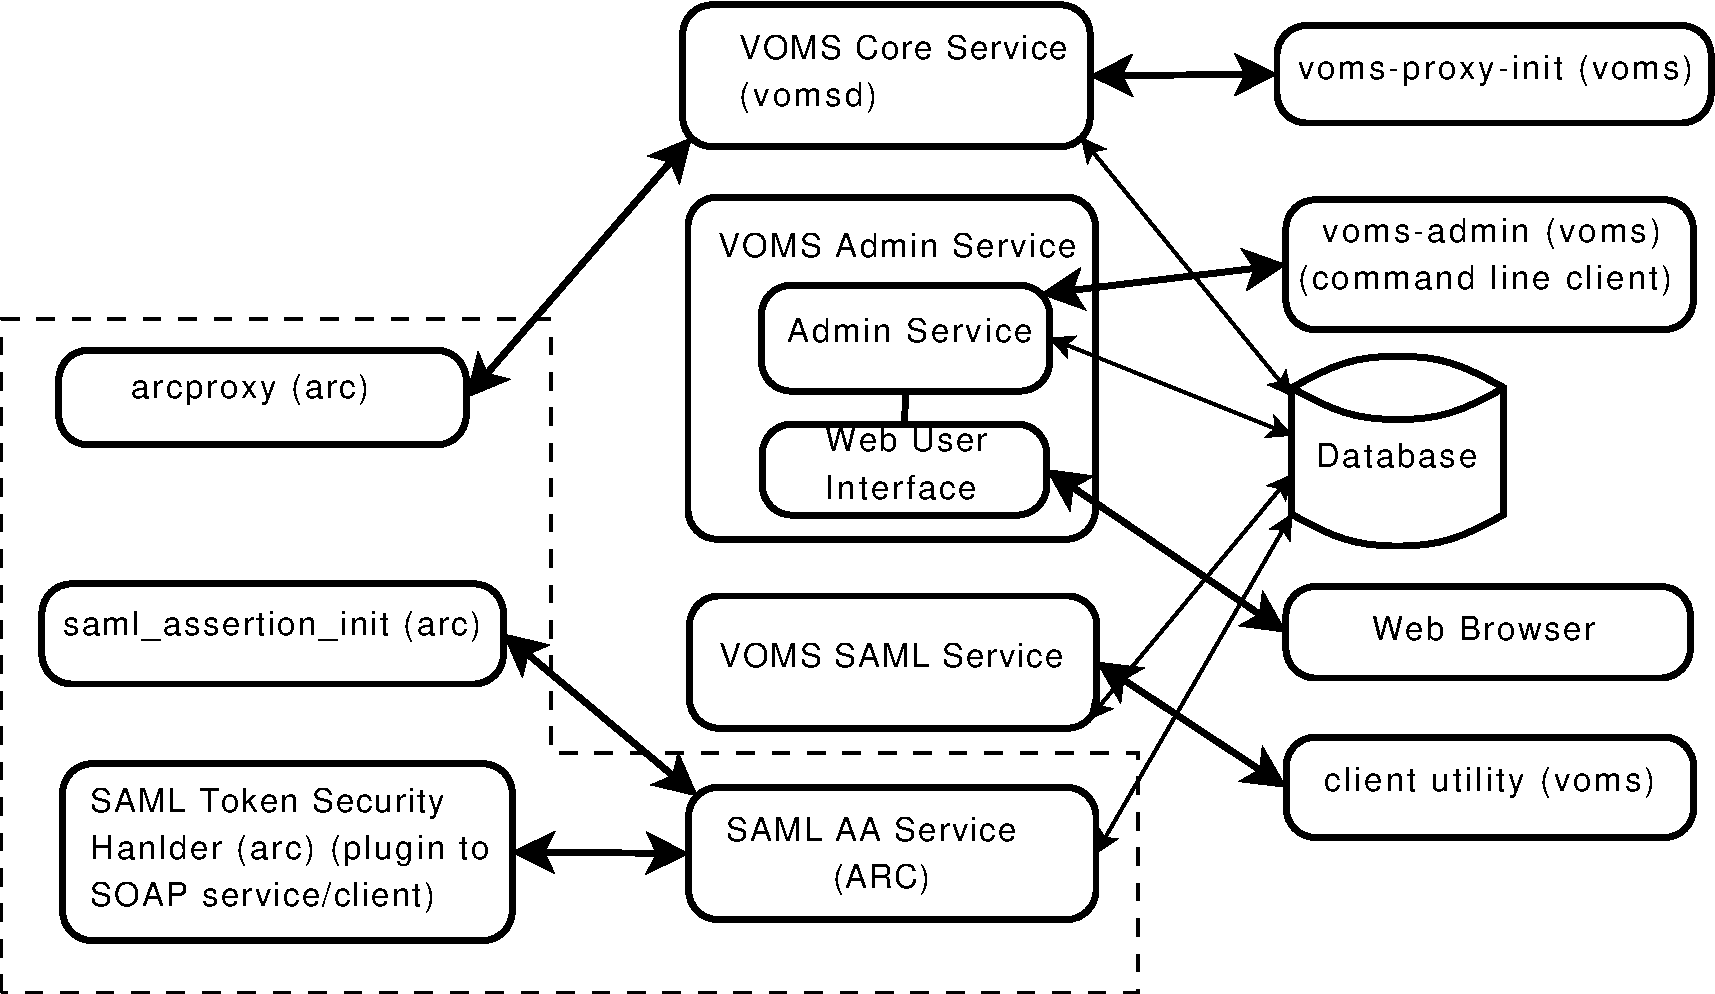
\includegraphics[width=1.0\textwidth]{arc_voms.pdf}}}
\caption{\label{fig:arc_voms}The relationship between ARC components and gLite (VOMS) components} }
\end{figure}

Howerver, the running of ARC's SAML AA Service does not neccessarily depend on VOMS Admin Service. As long as there is another attribute administration service (in parallel to VOMS Admin Service) which can nicely be used to manage the attributes, the SAML AA Service can be configured to adopt that service. The relationship between ARC's implementation and VOMS implementation is shown in \ref{fig:arc_voms}.

In terms of implementation, SAML AA Service in ARC is designed not to be coupled with any specific backend database schema. Therefore even if the database schema is changed, the implementation is not necessarily going to be changed. The way about decoupling the service implementation with database schema is through the service configuration.

\begin{verbatim}
    <samlp:AttributeQuery>
        <saml:Issuer/>
        <saml:Subject/>
        <saml:Attribute Name = "All">
        <saml:Attribute Name = "Role">
    <samlp:AttributeQuery>
\end{verbatim}

The following is the configuration about SAML AA Service, which uses the VOMS database schema when quering attributes.
The database query is distinguished by the ``\textit{name}'' attribute of $<$SQLSet$>$ element. If the ``\textit{Name}'' of $<$saml:Attribute$>$ (see the above for an example about \textit{$<$samlp:AttributeQuery$>$}) matches the ``\textit{name}'' attribute of $<$SQLSet$>$ element, then the corresponding \textit{SQL} under this $<$SQLSet$>$ element will be executed, and the result will be put into the SAML asserion.

\begin{verbatim}
        <Service name="aa.service" id="aa_service">
            <aa:KeyPath>../../tests/echo/testkey-nopass.pem</aa:KeyPath>
            <aa:CertificatePath>../../tests/echo/testcert.pem</aa:CertificatePath>
            <aa:CACertificatesDir>../../tests/echo/certificates</aa:CACertificatesDir>
            <aa:CACertificatePath>../../tests/echo/testcacert.pem</aa:CACertificatePath>

            <aa:Database type="mysql" ip="localhost" port="3305" dbname="voms_knowarc" user="root"
              password="123456">
              <!--The sql following sentences and their combination are introduced
              according to the code of voms' mysql plugin.
              The intention is that if some other database schema is used, you can
              simply change the sql sentences here, without changing the code. But still,
              the input argument to these queries should be with the same meaning,
              and the same sequence as the following; also the output of these queries
              should also be with the same meaning and the same sequence as the following-->
              <aa:SQLSet name="UID">
                <aa:SQL name="GetUID">SELECT userid FROM usr WHERE usr.dn = ?</aa:SQL>
              </aa:SQLSet>

              <aa:SQLSet name="Role">
                <aa:SQL name="GetRole">SELECT groups.dn, role FROM groups,
                  m LEFT JOIN roles ON roles.rid = m.rid WHERE groups.gid = m.gid
                  AND m.userid = ? AND roles.role = ?</aa:SQL>
                <aa:SQL name="GetGroup">SELECT groups.dn, NULL FROM groups, m
                  WHERE groups.gid = m.gid AND m.userid = ?</aa:SQL>
              </aa:SQLSet>

              <aa:SQLSet name="Group">
                <aa:SQL name="GetGroup">SELECT groups.dn, NULL FROM groups, m
                  WHERE groups.gid = m.gid AND m.userid = ?</aa:SQL>
              </aa:SQLSet>

              <aa:SQLSet name="GroupAndRole">
                <aa:SQL name="GetGroup">SELECT groups.dn, NULL FROM groups, m
                  WHERE groups.gid = m.gid AND m.userid = ?</aa:SQL>
                <aa:SQL name="GetGroupAndRole">SELECT groups.dn, role FROM groups,
                  m LEFT JOIN roles ON roles.rid = m.rid WHERE groups.gid = m.gid
                  AND m.userid = ? AND roles.role = ? AND groups.dn = ?</aa:SQL>
              </aa:SQLSet>

              <aa:SQLSet name="All">
                <aa:SQL name="GetAll">SELECT groups.dn, role FROM groups,
                  m LEFT JOIN roles ON roles.rid = m.rid WHERE groups.gid = m.gid
                  AND m.userid = ?</aa:SQL>
              </aa:SQLSet>

              <aa:SQLSet name="GroupAndRoleAttribute">
                <aa:SQL name="GetUserAttribute">SELECT attributes.a_name,
                  usr_attrs.a_value, NULL, NULL FROM attributes, usr_attrs
                  WHERE attributes.a_id = usr_attrs.a_id AND usr_attrs.u_id = ?
                </aa:SQL>
                <aa:SQL name="GetGroupAttribute">SELECT attributes.a_name,
                  group_attrs.a_value, groups.dn, NULL FROM attributes, group_attrs,
                  groups, m WHERE attributes.a_id = group_attrs.a_id AND groups.gid = m.gid
                  AND m.userid = ? AND m.rid is NULL AND group_attrs.g_id = m.gid
                </aa:SQL>
                <aa:SQL name="GetGroupAndRoleAttribute">SELECT attributes.a_name,
                  role_attrs.a_value, groups.dn, roles.role FROM attributes, role_attrs,
                  groups, roles, m WHERE attributes.a_id = role_attrs.a_id
                  AND groups.gid = m.gid AND m.userid = ? AND m.rid = roles.rid
                  AND roles.role = ? AND groups.dn = ? AND role_attrs.g_id = m.gid
                  AND role_attrs.r_id = m.rid
                </aa:SQL>
              </aa:SQLSet>

              <aa:SQLSet name="GroupAttribute">
                <aa:SQL name="GetUserAttribute">SELECT attributes.a_name,
                  usr_attrs.a_value, NULL, NULL FROM attributes, usr_attrs
                  WHERE attributes.a_id = usr_attrs.a_id AND usr_attrs.u_id = ?
                </aa:SQL>
                <aa:SQL name="GetGroupAttribute">SELECT attributes.a_name,
                  group_attrs.a_value, groups.dn, NULL FROM attributes, group_attrs,
                  groups, m WHERE attributes.a_id = group_attrs.a_id AND groups.gid = m.gid
                  AND m.userid = ? AND m.rid is NULL AND group_attrs.g_id = m.gid
                </aa:SQL>
              </aa:SQLSet>

              <aa:SQLSet name="RoleAttribute">
                <aa:SQL name="GetUserAttribute">SELECT attributes.a_name,
                  usr_attrs.a_value, NULL, NULL FROM attributes, usr_attrs
                  WHERE attributes.a_id = usr_attrs.a_id AND usr_attrs.u_id = ?
                </aa:SQL>
                <aa:SQL name="GetRoleAttribute">SELECT attributes.a_name,
                  role_attrs.a_value, groups.dn, roles.role FROM m
                  INNER JOIN groups ON m.gid = groups.gid LEFT JOIN roles
                  ON roles.rid = m.rid INNER JOIN role_attrs on groups.gid = role_attrs.g_id
                  INNER JOIN attributes on attributes.a_id = role_attrs.a_id
                  WHERE role_attrs.r_id = roles.rid AND m.userid = ? AND roles.role = ?
                </aa:SQL>
              </aa:SQLSet>

              <aa:SQLSet name="AllAttribute">
                <aa:SQL name="GetUserAttribute">SELECT attributes.a_name,
                  usr_attrs.a_value, NULL, NULL FROM attributes, usr_attrs
                  WHERE attributes.a_id = usr_attrs.a_id AND usr_attrs.u_id = ?
                </aa:SQL>
                <aa:SQL name="GetGroupAttribute">SELECT attributes.a_name,
                  group_attrs.a_value, groups.dn, NULL FROM attributes, group_attrs,
                  groups, m WHERE attributes.a_id = group_attrs.a_id AND groups.gid = m.gid
                  AND m.userid = ? AND m.rid is NULL AND group_attrs.g_id = m.gid
                </aa:SQL>
                <aa:SQL name="GetGroupAndRoleAttributeAll">SELECT attributes.a_name,
                  role_attrs.a_value, groups.dn, roles.role FROM attributes, role_attrs,
                  groups, roles, m WHERE attributes.a_id = role_attrs.a_id
                  AND groups.gid = m.gid AND m.userid = ? AND m.rid = roles.rid
                  AND role_attrs.g_id = m.gid AND role_attrs.r_id = m.rid
                </aa:SQL>
              </aa:SQLSet>

              <aa:SQLSet name="Default">
                <aa:SQL name="GetDefault">SELECT groups.dn, role FROM groups,
                  m LEFT JOIN roles ON roles.rid = m.rid WHERE groups.gid = m.gid
                  AND m.userid = ?</aa:SQL>
              </aa:SQLSet>
              <!--Other SQLSet-->

            </aa:Database>
        </Service>
\end{verbatim}

The configuration of SAML AA service is according to the schema:

http://svn.nordugrid.org/trac/nordugrid/browser/arc1/trunk/src/services/saml/aaservice.xsd

%section saml_aa_service (end)

\bibliography{grid}

\end{document}
